\documentclass[9pt]{beamer}
\usepackage[sfdefault]{roboto}
\usepackage{styles/fluxmacros}
\usefolder{styles}
\usetheme[style=asphalt]{flux}
\usepackage{xcolor}
\usepackage{color}
\usepackage{amsmath}
\usepackage{amssymb}
\usepackage{graphicx}
\usepackage{latexsym}
\usepackage[T1]{fontenc}
\usepackage[utf8]{inputenc}
\usepackage{wrapfig}
\usepackage{siunitx}
\usepackage{times}
\usepackage{tikz}
\usepackage{verbatim}
\usepackage{multimedia}
\usepackage{hyperref}
\usepackage{thumbpdf}
\usepackage{pgf,pgfarrows,pgfnodes,pgfautomata,pgfheaps,pgfshade}
\usepackage{url}
\usepackage{empheq}
\usepackage{fancybox}
\usepackage{esint}
\usepackage{lipsum}
\usepackage{listings}
\usepackage{mathptmx}
\usepackage{helvet}
\usepackage{tikz}%
\usepackage{circuitikz}
\usepackage{csvsimple}
\usepackage{pgfplots}
\usepackage{multimedia}
\usepackage{proba}
\usepackage[absolute,overlay]{textpos}
\usepackage{bibunits}
\usepackage{tcolorbox}
\usepackage{qrcode}
%\usepackage[texcoord,
%            grid,
%            gridunit=mm,
%            gridcolor=red!60,
%            subgridcolor=black!60]{eso-pic}
\usepackage{enumerate}
\setbeamercovered{transparent}
%% Informations
\usepackage[makeroom]{cancel}
\usepackage{epstopdf}
\usepackage{booktabs}
\usepackage{calc}  
\usepackage{enumitem} 
\epstopdfsetup{outdir=./}
\mode<presentation>
{
    %\usetheme{PaloAlto}
    %\usecolortheme[named=kugreen]{structure}
    \useinnertheme{progressbar}
    %\usefonttheme{default}
    %\usefonttheme{serif}
    %\setbeamercovered{transparent}
    %\setbeamertemplate{blocks}[rounded][shadow=true]
    %\setbeamertemplate{navigation symbols}[only frame symbol]
}
\setbeamertemplate{items}[ball]
%
%
%~~~~~~~~~~~~~~~~~~~~~~~~~~~~~~~~~~~~~~~~~~~~~~~~~~~~~~~~~~~~~~~~~~~~~~~~~~~~~~
%~~~~~~~~~~~~~~~~~~~~~~~~~~~~~~~~~~~~~~~~~~~~~~~~~~~~~~~~~~~~~~~~~~~~~~~~~~~~~~
% Informations
\defaultbibliography{main}
%
%
%
\title{\Huge{COVID-19 optimal vaccination policies:}}
\subtitle{%
    \huge{A modeling study on efficacy,}
    \\
    \huge{
        \textbf{
            \textcolor{gray}{
                 natural and vaccine-induced immunity%
            }
        }
    }
    \\
    \huge{
        \textbf{
            \textcolor{gray}{
                 responses,%
            }
        }
    } \normalsize{\today}
}
%
\author{
    \normalsize{CONACYT-UNISON-ITSON Mathematical biology group}
}
%
\date{June 23 2021}

\titlegraphic{assets/logoSIAM.png}
%~~~~~~~~~~~~~~~~~~~~~~~~~~~~~~~~~~~~~~~~~~~~~~~~~~~~~~~~~~~~~~~~~~~~~~~~~~~~~~
%%%%%%%%%%%%%%%%%%%%%%%%%%%%%%%%%%%%%%%%%%%%%%%%%%%%%%%%%%%%%%%%%%%%%%%%%%%%%%%%
\def\Q#1#2{\frac{\partial #1}{\partial #2}}
\usetikzlibrary{arrows,shapes}
\pgfplotsset{compat=1.14}
%%%%%%%%%%%%%%%%%%%%%%%%%%%%%%%%%%%%%%%%%%%%%%%%%%%%%%%%%%%%%%%%%%%%%%%%%%%%%%%%
%-----------------------------ExtrasDeTercerPresentacion
%--------------------------------Fancyboxes-------------------------------------
\definecolor{myblue}{rgb}{.8, .8, 1}
\definecolor{azure(colorwheel)}{rgb}{0.0, 0.5, 1.0}
\definecolor{shadecolor}{cmyk}{0,0,0.41,0}
\newcommand*\mybluebox[1]{%
    \colorbox{myblue}{\hspace{1em}#1\hspace{1em}}
}
\newcommand*\myyellowbox[1]{%
    \colorbox{darkyellow}{\hspace{1em}#1\hspace{1em}}
}
%--------------------------------------------------------------------------
\definecolor{shadecolor}{cmyk}{0,0,0.41,0}
\definecolor{light-blue}{cmyk}{0.25,0,0,0}
\newsavebox{\mysaveboxM} % M for math
\newsavebox{\mysaveboxT} % T for text
\newcommand*\Garybox[2][Example]{%
    \sbox{\mysaveboxM}{#2}%
        \sbox{\mysaveboxT}{\fcolorbox{black}{light-blue}{#1}}%
            \sbox{\mysaveboxM}{%
    \parbox[b][\ht\mysaveboxM+.5\ht\mysaveboxT+.5\dp\mysaveboxT][b]{%
        \wd\mysaveboxM}{#2}%
    }%
    \sbox{\mysaveboxM}{%
        \fcolorbox{black}{shadecolor}{%
        \makebox[\linewidth-10em]{\usebox{\mysaveboxM}}%
        }%
    }%
    \usebox{\mysaveboxM}%
    \makebox[0pt][r]{%
        \makebox[\wd\mysaveboxM][c]{%
            \raisebox{\ht\mysaveboxM-0.5\ht\mysaveboxT
            +0.5\dp\mysaveboxT-0.5\fboxrule}{\usebox{\mysaveboxT}}%
        }%
    }%
}
\newcommand\Fontvi{\fontsize{7}{7.2}\selectfont}
%%%%%%%%%%%%%%%%%%%%%%%%%%%%%%%%%%%%%%%%%%%%
\definecolor{kugreen}{RGB}{50,93,61}
\definecolor{kugreenlys}{RGB}{132,158,139}
\definecolor{kugreenlyslys}{RGB}{173,190,177}
\definecolor{kugreenlyslyslys}{RGB}{214,223,216}
\definecolor{greenArea}{RGB}{124,252,124}
\definecolor{hellmagenta}{rgb}{1,0.75,0.9}
\definecolor{hellcyan}{rgb}{0.75,1,0.9}
\definecolor{hellgelb}{rgb}{1,1,0.8}
\definecolor{colKeys}{rgb}{0,0,1}
\definecolor{colIdentifier}{rgb}{0,0,0}
\definecolor{colComments}{rgb}{1,0,0}
\definecolor{colString}{rgb}{0,0.5,0}
\definecolor{darkyellow}{rgb}{1,0.9,0}
\setbeamercovered{transparent}
\lstset{%
    language=[AlLaTeX]TEX,%
    float=hbp,%
    basicstyle=\ttfamily\small, %\usepackage{cir}
    identifierstyle=\color{colIdentifier}, %
    keywordstyle=\color{colKeys}, %
    stringstyle=\color{colString}, %
    commentstyle=\color{colComments}, %
    columns=flexible, %
    tabsize=3, %
    frame=single, %
    extendedchars=true, %
    showspaces=false, %
    showstringspaces=false, %
    numbers=left, %
    numberstyle=\tiny, %
    breaklines=true, %
    backgroundcolor=\color{hellgelb}, %
    breakautoindent=true, %
    captionpos=b,%
    xleftmargin=18pt,%
    xrightmargin=\fboxsep%
}
\pgfplotsset{
    left segments/.code={\pgfmathsetmacro\leftsegments{#1}},
    left segments=3,
    left/.style args={#1:#2}{
        ybar interval,
        domain=#1:#2,
        samples=\leftsegments+1,
        x filter/.code=\pgfmathparse{\pgfmathresult}
       }
}
\DeclareMathOperator{\sign}{sgn}
\newcommand{\innerprod}[2]{\left\langle#1, #2\right\rangle}
\newcommand\bound{10} % bound number of points on each side of N
\newcommand\labelnum[3][]{
    \begin{scope}[font=\footnotesize,x=.3cm,#1]
      \foreach \mypt in {0,#2,...,\bound}{
        \draw(\mypt,0)circle[radius=2pt];
        \draw(-\mypt,0)circle[radius=2pt];
      }
      \draw(-\bound-5,0)--(\bound+5,0) node[pos=0, left]{$t$};
      \node(start)[at={(-\bound-4,0)},label=below:{$t_0=0$}]{$[$};
      \node(end)[at={(\bound+4,0)},label=below:{$T=Nh$}]{$]$};
      \node[%
          at={($(start)!.319!(end)$)},
          label=below:{
               $\underbrace{}_{h}$
            }%
            ]{\vphantom{$[$}};
      \node[at={($(start)!.57!(end)$)},label=below:{$t_{n+1}$}]{\vphantom{$[$}};
      \filldraw(0,0)circle[radius=2pt];
      \node[at={(-\bound-2,0)},above]{$\cdots$};
      \node[at={(\bound+2,0)},above]{$\cdots$};
      \node[at={(0,0)},above=5pt]{#3};
    \end{scope}
}
\usepackage{remreset}
\makeatletter
\@removefromreset{subsection}{section}
\makeatother
\definecolor{greenstrong}{rgb}{0.58,0.77,0.29}
\definecolor{redstrong}{rgb}{0.81,0.22,0.23}
\definecolor{fglisting}{gray}{0.3}
\definecolor{bglisting}{gray}{1}
\definecolor{fgshell}{gray}{1}
\definecolor{bgshell}{gray}{0.1}
\definecolor{bgshelllight}{gray}{0.8}
\definecolor{cadmiumorange}{rgb}{0.93, 0.53, 0.18}
\definecolor{capri}{rgb}{0.0, 0.75, 1.0}
%
\setcounter{subsection}{1}
\newcommand{\hl}[1]{\textbf{\textcolor{greenstrong}{#1}}}
\newcommand{\hb}[1]{\textbf{\textcolor{azure(colorwheel)}{#1}}}
\newcommand{\hlErr}[1]{\textcolor{redstrong}{\texttt{#1}}}
\newcommand{\hlOk}[1]{\textcolor{green}{\texttt{#1}}}
\newcommand{\hlInv}[1]{\colorbox{bgshell}{\textcolor{fgshell}{\texttt{#1}}}}
\newcommand{\unhl}[1]{\textcolor{gray}{#1}}
\newcommand{\clda}[0]{$\textcolor{blue}{\lambda}$}
\newcommand{\carr}[0]{$\textcolor{purple}{\rightarrow}$}
\newcommand{\cbind}[0]{\textbf{\texttt{$>\!\!>\!\!=$}}}
\newcommand{\codedots}[0]{\textcolor{mid-gray}{...}}

%
\tcbuselibrary{skins, breakable}
\newtcolorbox{greenbox}[1]{%
        colback = green!5!white,
        colframe = green!55!black,
        fonttitle = \bfseries,
        title = #1 %
    }
\newtcolorbox{bluebox}[1]{%
        colback = blue!5!white,
        colframe = blue!55!black,
        fonttitle = \bfseries,
        title = #1
    }
%
\newtcolorbox{graybox}[1]{%
        colback = gray!5!white,
        colframe = gray!55!black,
        fonttitle = \bfseries,
        title = #1
    }
%
\newtcolorbox{yellowbox}[1]{%
        colback = yellow!5!white,
        colframe = yellow!55!black,
        fonttitle = \bfseries,
        title = #1
    }

\newcolumntype{P}[1]{>{\centering\arraybackslash}p{#1}}
\begin{document}
    \titlepage
    \section*{Introduction}
        %!TEX root = ../main.tex
\begin{frame}{Toy example and classic vaccination OC}
    \setlength{\leftmargini}{1mm}
    \begin{textblock*}{65mm}(0mm, 10mm)
        \only<1->{
            To fix ideas:
            \begin{equation*}
                \begin{aligned}
                   S'(t) &= -\beta IS
                   \\
                   I'(t) &=  \beta IS - \gamma I
                   \\
                   R'(t) & = \gamma I
                   \\
                   & S(0) = S_0, I(0)=I_0, R(0)=0 
                   \\
                   & S(t) + I(t) + R(t )= 1
                \end{aligned}
            \end{equation*}
        }
     \end{textblock*}
     %
    \begin{textblock*}{65mm}(65mm, 10mm)
        \only<2>{
            With vaccination
            \begin{equation*}
                \begin{aligned}
                   S'(t) &= -\beta IS  - \textcolor{red}{\lambda_V(t)}
                   \\
                   I'(t) &=  \beta IS - \gamma I
                   \\
                   R'(t) & = \gamma I
                   \\
                   V'(t) & = \textcolor{red}{\lambda_V(t)}
                   \\
                   & S(0) = S_0, I(0)=I_0, 
                   \\
                   &R(0)=0, V(0) = 0
                   \\
                   & S(t) + I(t) + R(t) + V(t)= 1
                \end{aligned}
            \end{equation*}
        }
     \end{textblock*}
     \begin{textblock*}{65mm}(65mm, 10mm)
        \only<3->{
            \begin{equation*}
                \begin{aligned}
                   S'(t) &= -\beta IS  - \textcolor{red}{\lambda_V(x, t)}
                   \\
                   I'(t) &=  \beta IS - \gamma I
                   \\
                   R'(t) & = \gamma I
                   \\
                   V'(t) & = \textcolor{red}{\lambda_V(x,t)}
                   \\
                   & S(0) = S_0, I(0)=I_0, 
                   \\
                   &R(0)=0, V(0)=0
                   \\
                   & S(t) + I(t) + R(t) + V(t)= 1
                   \\
                   & x^{\top}=(S,I,R,V)
                \end{aligned}
            \end{equation*}
        }
     \end{textblock*}
     \begin{textblock*}{28mm}(5mm, 45mm)
        \begin{block}{``Classic'' Vaccination}
            \begin{itemize}          
                \item
                \only<4->{
                    Gumel,
                }
                \only<6->{
                    $$
                        \lambda_V:= 
                        \underbrace{ \textcolor{orange}{\xi}}_{cte.}
                        \cdot \ S(t)
                    $$
                }
                
            \end{itemize}
            \only<7->{
                Optimal Controlled:
            }
        \end{block}
     \end{textblock*}
     \begin{textblock*}{80mm}(45mm,48mm)
        \only<6>{
        \begin{bibunit}[apalike]
            \nocite{Alexander2004,Iboi2020}
            \putbib
        \end{bibunit}
        }
        \only<7>{
        \begin{bibunit}[apalike]
            \nocite{Hethcote1973,Wickwire1977}
            \putbib
        \end{bibunit}
        }
     \end{textblock*}
 \end{frame}
%%%%%%%%%%%%%%%%%%%%%%%%%%%%%%%%%%%%%%%%%%%%%%%%%%%%%%%%%%%%%%%%%%%%%%%%%%%%%%
\begin{frame}{The Basic Optimization Question}
    \setlength{\leftmargini}{1mm}
    \begin{textblock*}{72.5mm}(0mm, 10mm)
        \begin{graybox}{Hypothesis}
            \begin{description}[leftmargin=!,
            labelwidth=\widthof{\bfseries Jabs Counter}]

                \only<1->{
                \item[Cost]
                    The \textbf{effort} expended in 
                    ``\textbf{preventing-mitigating}
                    an epidemic'' by vaccination is 
                    \textbf{proportional} to the vaccination
                    rate $\lambda_V$.
                }
                %
                \only<2->{
                \item[Jabs Counter]
                    If $S(0)\approx 1$ , $X(\cdot):$ counts 
                    vaccine doses, then
                    $$
                    X(t) = 1 - \exp(-\lambda_V t),
                    $$
                    estimates the fraction of vaccinated 
                    individuals.
                    Thus, for time horizon $T$ and 
                    vaccination coverage %$X_{cov}$
                }
                    \only<3-6>{
                        \begin{equation*}
                            \begin{aligned}
                                X_{cov} &= X(T)
                                \\
                                &\approx 
                                    1 - \exp(-\textcolor{teal}{\lambda_V} T).
                            \end{aligned}
                        \end{equation*}
                    }
            \end{description}
        \end{graybox}
    \end{textblock*}
    \begin{textblock*}{50mm}(75mm, 10mm)
        \only<4->{
            \begin{yellowbox}{{Given $X_{cov}$, \ $T$}}
                $$
                    \lambda_V = -\frac{1}{T} 
                    \ln(1 - X_{cov})
                $$
                \textbf{estimates} the constant vaccination rate s.t., 
                afther time $T$, we reach $X_{cov}$.
            \end{yellowbox}
        }
        \only<5->{
            \begin{greenbox}{{$X_{COV}: 70 \%$, $T$: one \SI{}{year}}}
                $
                    \lambda_V \approx \num{0.00329}
                $
                \tcblower
                \only<6>{
                    If $S(0) N$ corresponds to HMS
                    (\SI{812229}{inhabitants})
                    $
                        % \num{0.00611352} \times \num{100000}
                        \approx \SI{2668}{jabs \per day}.
                    $
                }
                \only<7->{
                    \textcolor{orange}{
                    \textbf{
                        How to optimize vaccination?}
                    }
                }
            \end{greenbox}
        }
    \end{textblock*}
    %--------------------------------------------------------------------------
    \begin{textblock*}{62mm}(5mm, 70mm)
        \only<8->{
            \begin{block}{Common Objectives}
                \begin{itemize}
                    \item
                    \only<9->{
                       
                        Who to vaccine first?    
                        (Allocation) 
                    }
                    \item
                    \only<10->{
                        
                        How and when?
                        (Administration)
                    }
                \end{itemize}
            \end{block}
        }
    \end{textblock*}
\end{frame}
%%%%%%%%%%%%%%%%%%%%%%%%%%%%%%%%%%%%%%%%%%%%%%%%%%%%%%%%%%%%%%%%%%%%%%%%%%%%%%%
\begin{frame}{Vaccine optimiztion for COVID-19}
    \begin{textblock*}{50mm}(5mm, 10mm)
        \begin{block}{Common Objectives}
           \begin{itemize}[label=$\mathbf{\star}$]
                \item
                    \textcolor<5>{orange}{
                        Who to vaccine first?    
                        (Allocation)
                    } 
                \only<2->{
                    \item
                         \textcolor<6->{orange}{
                            How and when?
                            \textbf<7>{
                                (Administration)
                            }                
                         }
                }
            \end{itemize}
        \end{block}
    \end{textblock*}
%
    \begin{textblock*}{55mm}(65mm, 10mm)
        
        \only<2->{
            \begin{block}{%
                \only<2-3>{Cost}
                \only<4->{Optimal Control Problem}
            }
                \only<3>{
                    \begin{equation*}
                        \begin{aligned}
                            % \min_{\mathbf{u} \in \mathcal{U}}
                            J(u) := &
                            \varphi(x(T)) + 
                            \int_0 ^  T
                                f(t, x(t), u(t))
                        \end{aligned}
                    \end{equation*}
                }
                \only<4->{
                    \begin{equation*}
                        \begin{aligned}
                            \min_{\mathbf{u} \in \mathcal{U}}
                                J(u) = &
                                \varphi(x(T)) + 
                                \int_0 ^  T
                                    f(t, x(t), u(t))
                            \\
                            \dot{x}(t) =& b(t,u(t), x(t)), 
                            \qquad \text{a.e. }t \in[0,T],
                            \\
                                x(0)=& x_0
                        \end{aligned}
                    \end{equation*}
                }
            \end{block}
        }
    \end{textblock*}
    %
    \begin{textblock*}{115mm}(10mm, 42mm)
        \only<5>{
            \begin{bibunit}[apalike]
                \nocite{Matrajt2020,Bubar2020,Buckner2020}
                \putbib
            \end{bibunit}
        }
        \only<6-7>{
        \begin{bibunit}[apalike]
            \nocite{Zegarra2020, Salcedo-Varela2021}
            \putbib
        \end{bibunit}
        }
        \only<8>{
            \begin{textblock*}{65mm}(30mm, 55mm)
                \begin{yellowbox}{Aim of this talk}
                    To illustrate the formulation of optimal vaccination policies
                    based in vaccination rate.
                \end{yellowbox}
            \end{textblock*}
        }   
    \end{textblock*}
\end{frame}
    \section{The model without vaccination}
        %!TEX root = ../main.tex
\begin{frame}{Model Scheme}
    \setlength{\leftmargini}{1mm}
    %!TEX root = ../main.tex
        \setlength{\leftmargini}{1mm}
        \begin{textblock*}{65mm}(5mm, 10mm)
            \only<1>{
                \includegraphics[scale=0.125,%
                    keepaspectratio]{assets/%
                    SchemeModel_withoutVaccination.png}
            }
            \only<2>{
                \includegraphics[scale=0.125,%
                    keepaspectratio]{assets/%
                    SchemeModel_withoutVaccination00.png}
            }
            \only<3->{
                \includegraphics[scale=0.125,%
                    keepaspectratio]{assets/%
                    SchemeModel_withoutVaccination01.png}
            }
        \end{textblock*}
%
    \begin{textblock*}{45mm}(82mm, 55mm)
        \only<2-4>{
            \begin{bluebox}{Vaccine Hypotheses}
                \begin{itemize}
                    %TODO: change bullet indentation
                    \item
                        Imperfect preventive
                    \item
                        One dose
                    \item
                        Symptomatic exception
                    \item
                        Action over susceptible
                \end{itemize}
            \end{bluebox}
        }
    \end{textblock*}
    \begin{textblock*}{75mm}(5mm, 65mm)
    \only<4->{
        \begin{bluebox}{Notation}
            \begin{tabular}{rl}
                $\epsilon$
                & vaccine efficacy 
                \\
                $p$
                & Generation of symptoms  probability
                % \\
                % $u_V(t)$
                % & Optimal vaccination policy
            \end{tabular}
        \end{bluebox}
        }
    \end{textblock*}
%
    \begin{textblock*}{45mm}(82mm, 50mm)
        \only<5->{
            \begin{bluebox}{SAGE objectives}
                \begin{itemize}
                    \item
                        Vaccine profile \\(Efficacy, immunity)
                    \item
                        Coverage
                    \item
                        Time Horizon
                \end{itemize}
                \tcblower
                \only<6->{
                    Immunity:
                    \begin{itemize}
                        \item
                            natural (reinfection)
                        \item
                            vaccine-induced 
                    \end{itemize}
                }
            \end{bluebox}
        }
    \end{textblock*}
\end{frame}
    \section{Reproductive Vaccination Number}
        %!TEX root = ../main.tex
\begin{frame}{Reproductive number}
    \setlength{\leftmargini}{1mm}
    \begin{textblock*}{65mm}(0mm, 25mm)
        \only<1>{
            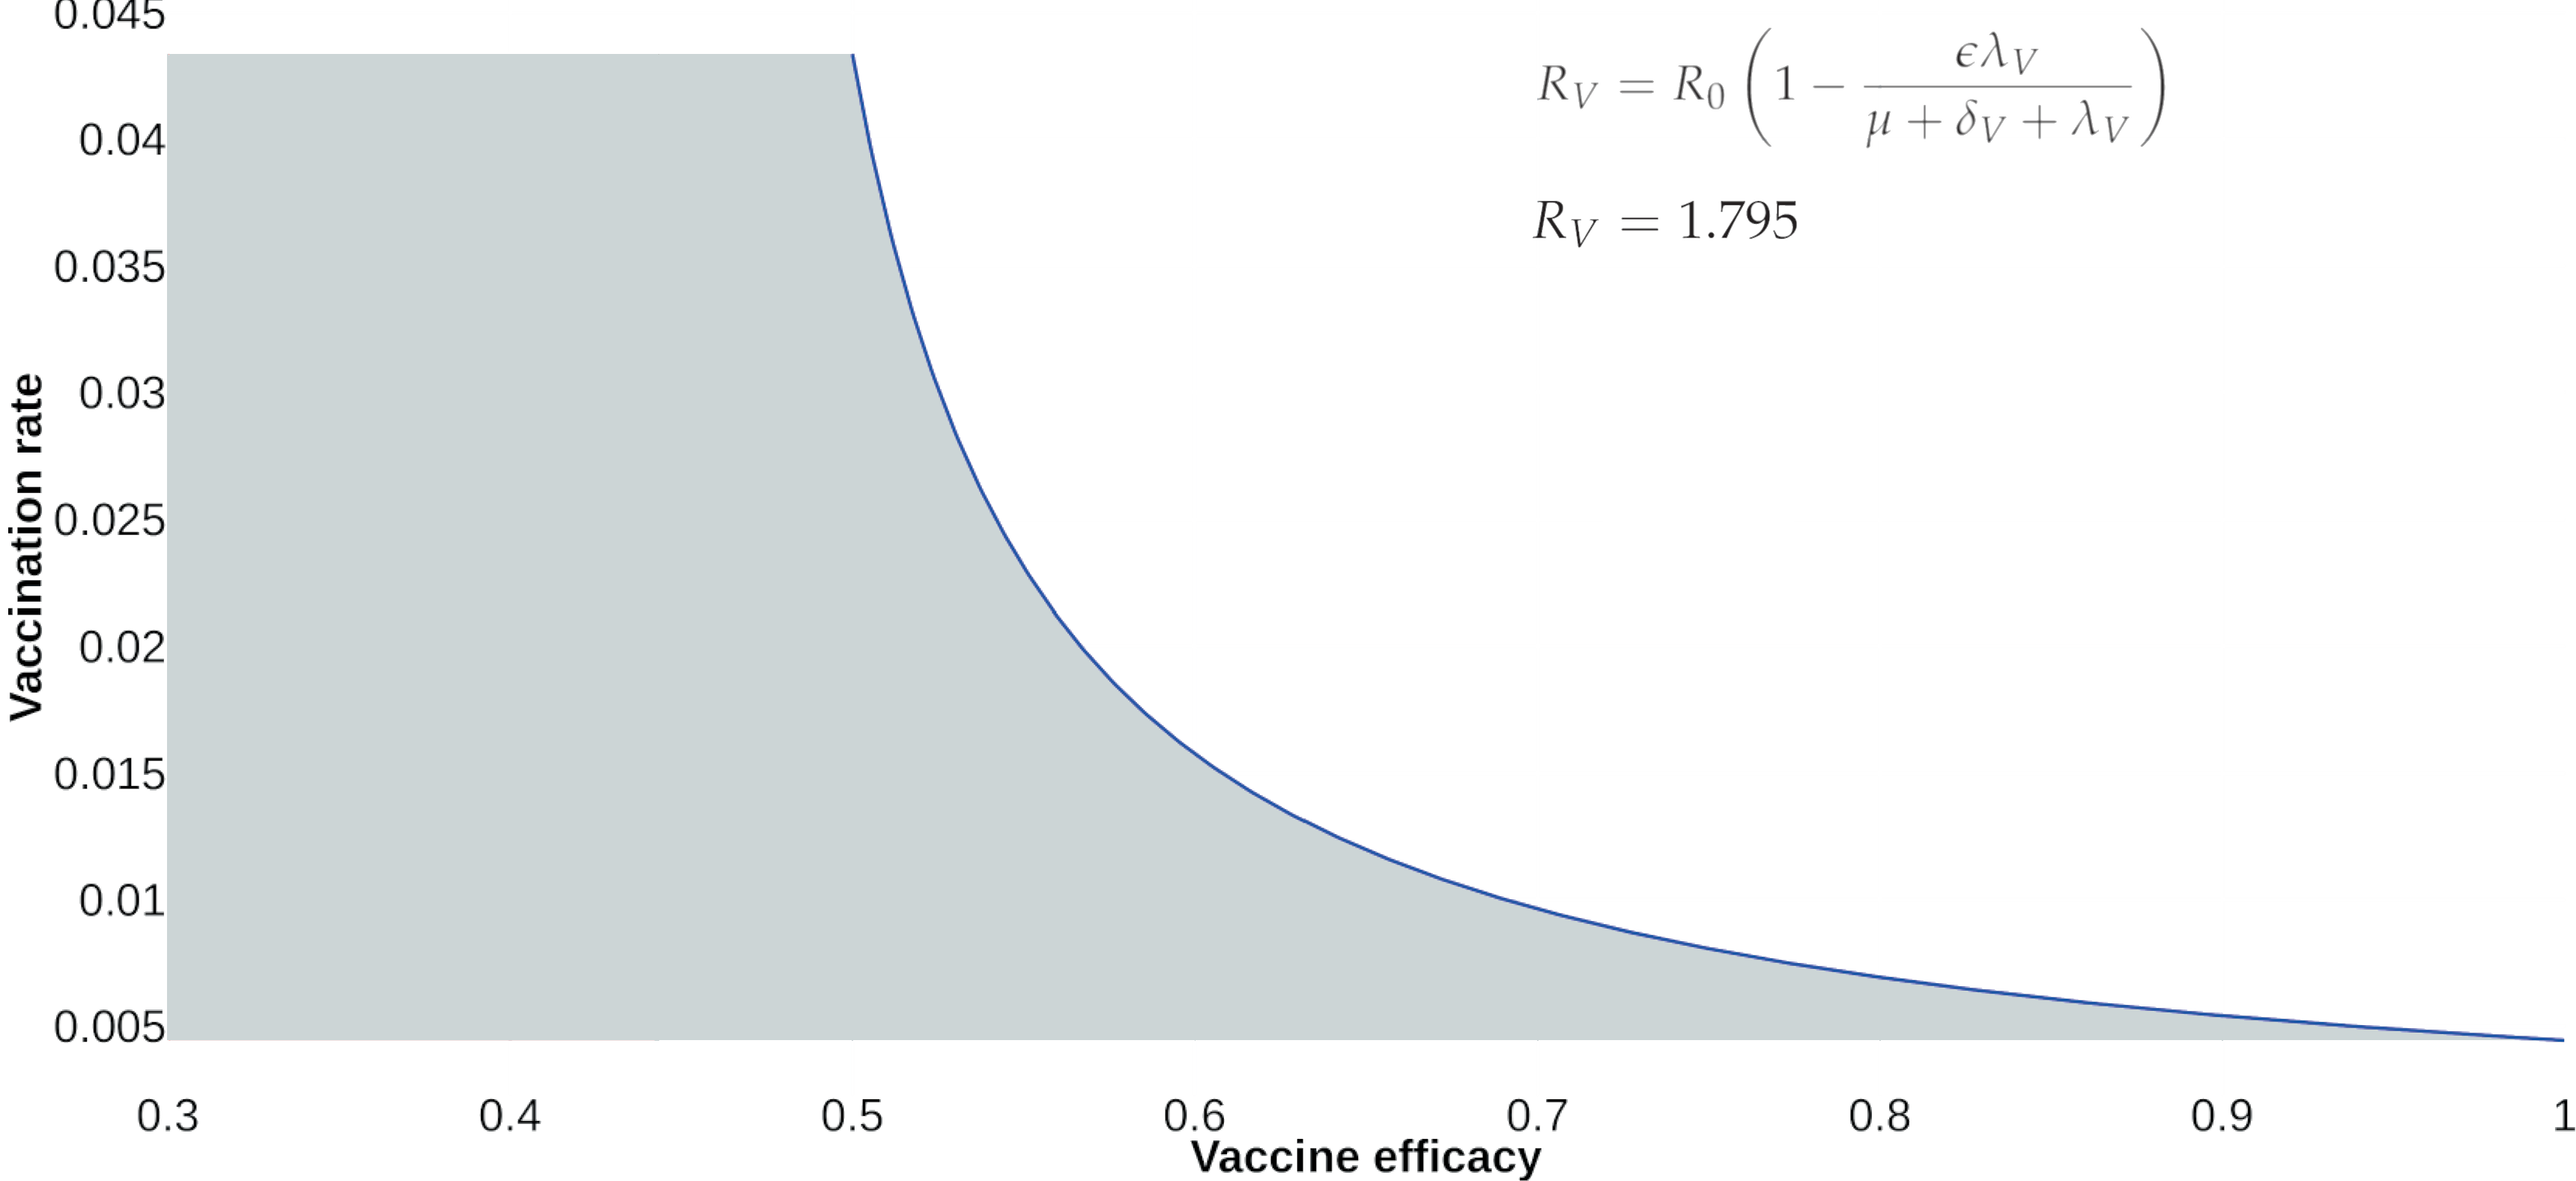
\includegraphics[scale=.875,%
                keepaspectratio]{assets/RvAnimation//r_zero_vac_efficiency01.png}
        }
        \only<2>{
            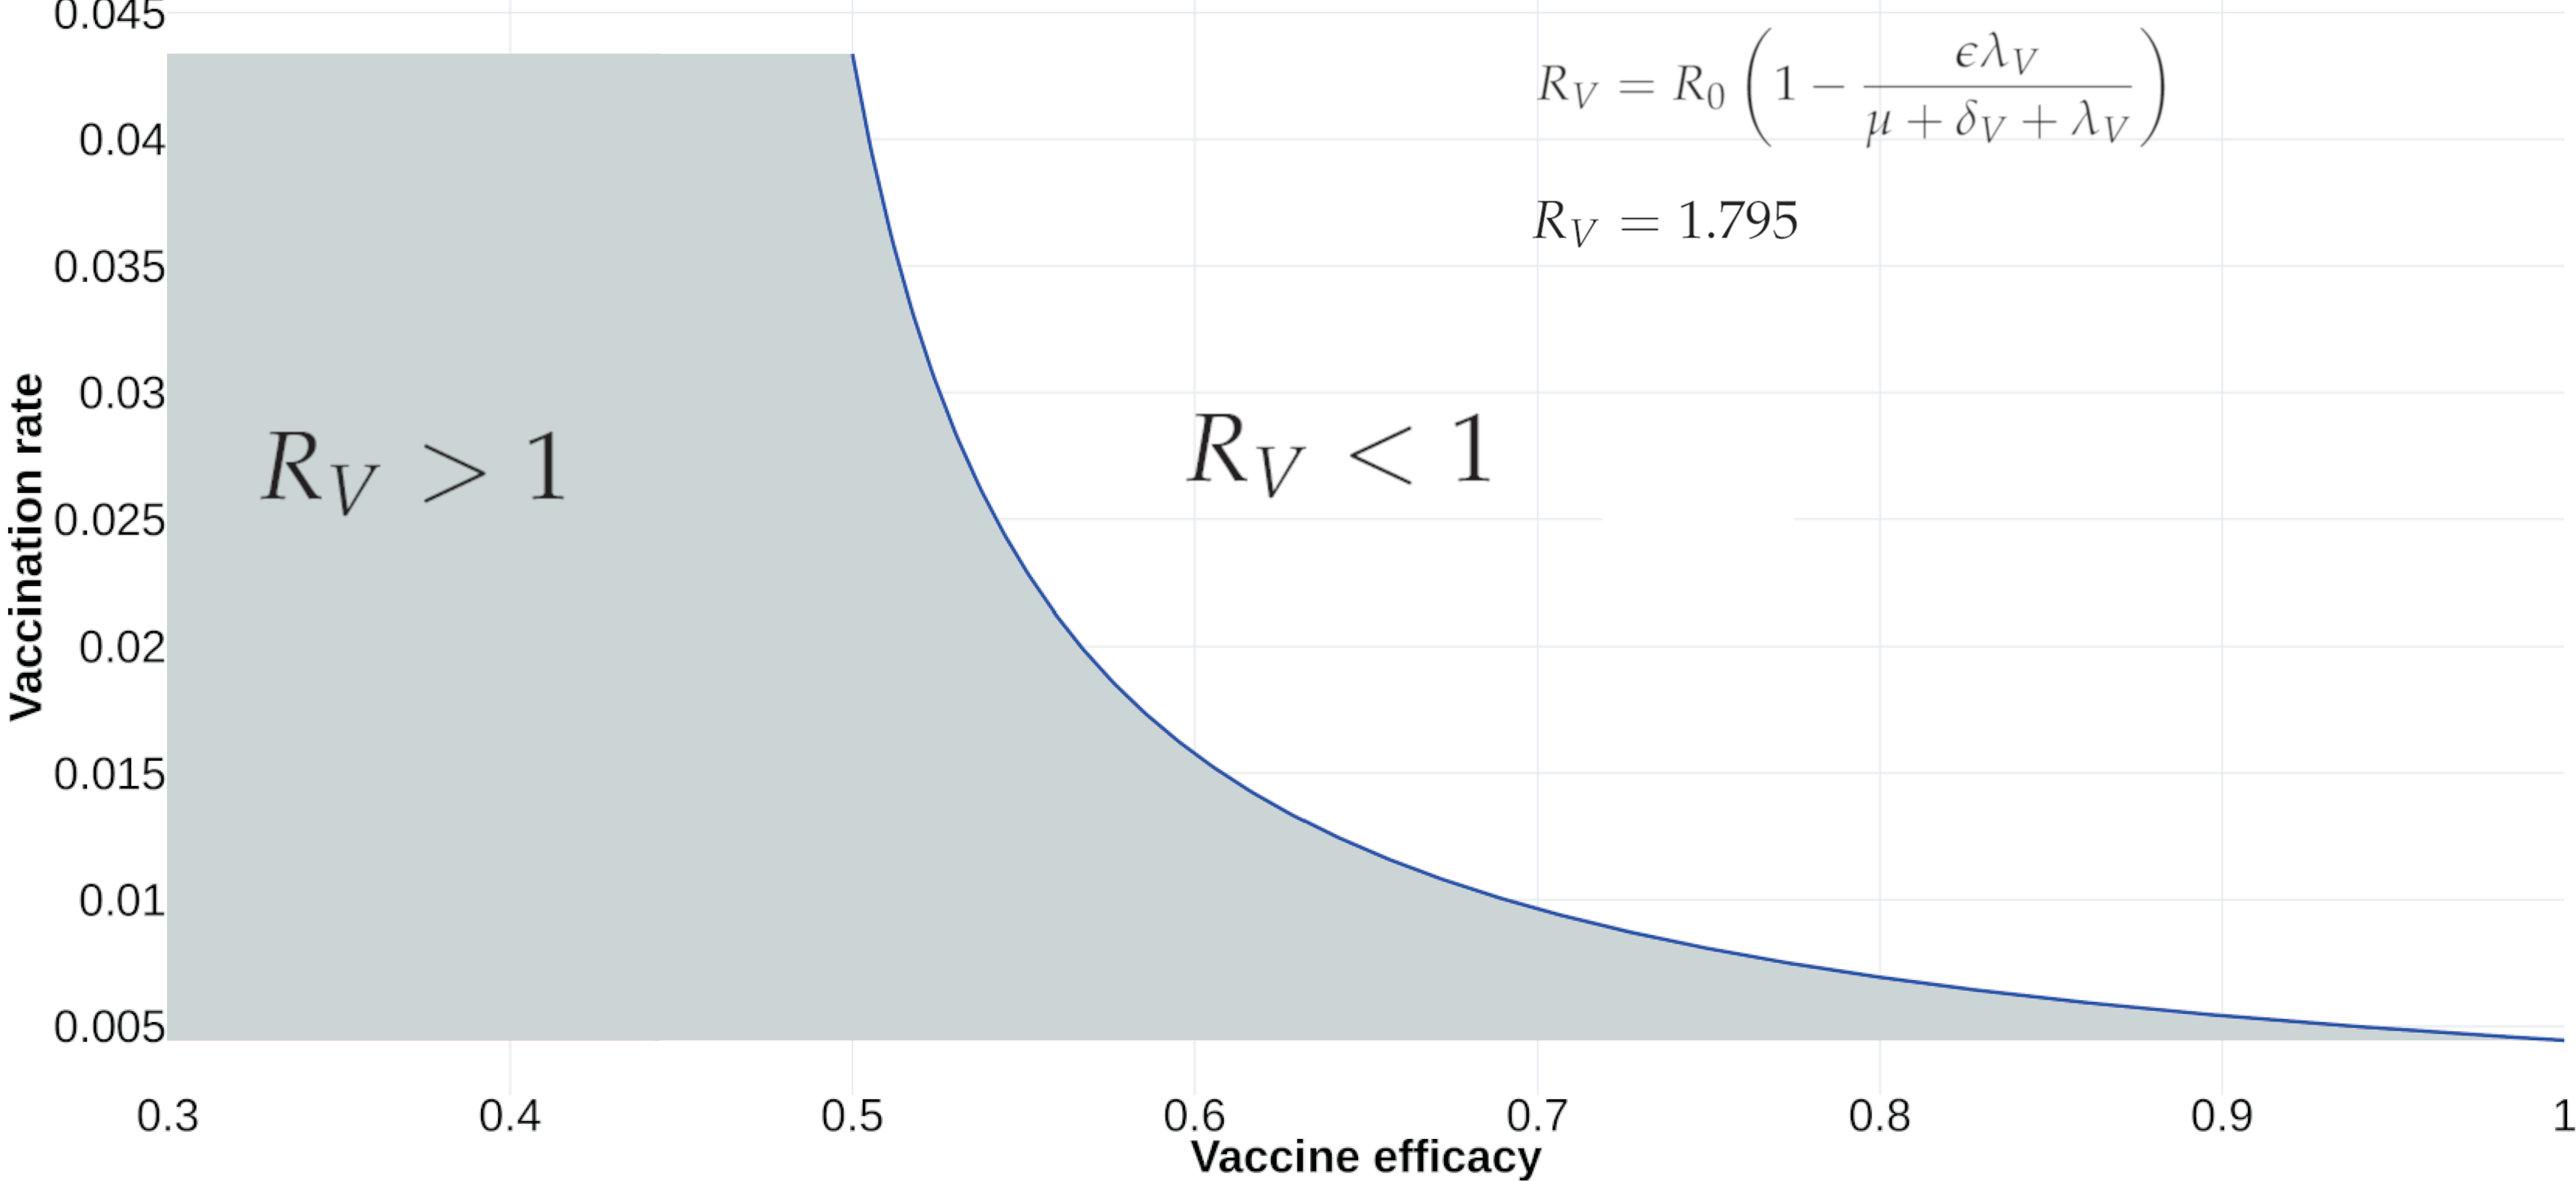
\includegraphics[scale=.875,%
            keepaspectratio]{assets/RvAnimation//r_zero_vac_efficiency02.png}
        }
        \only<3>{
            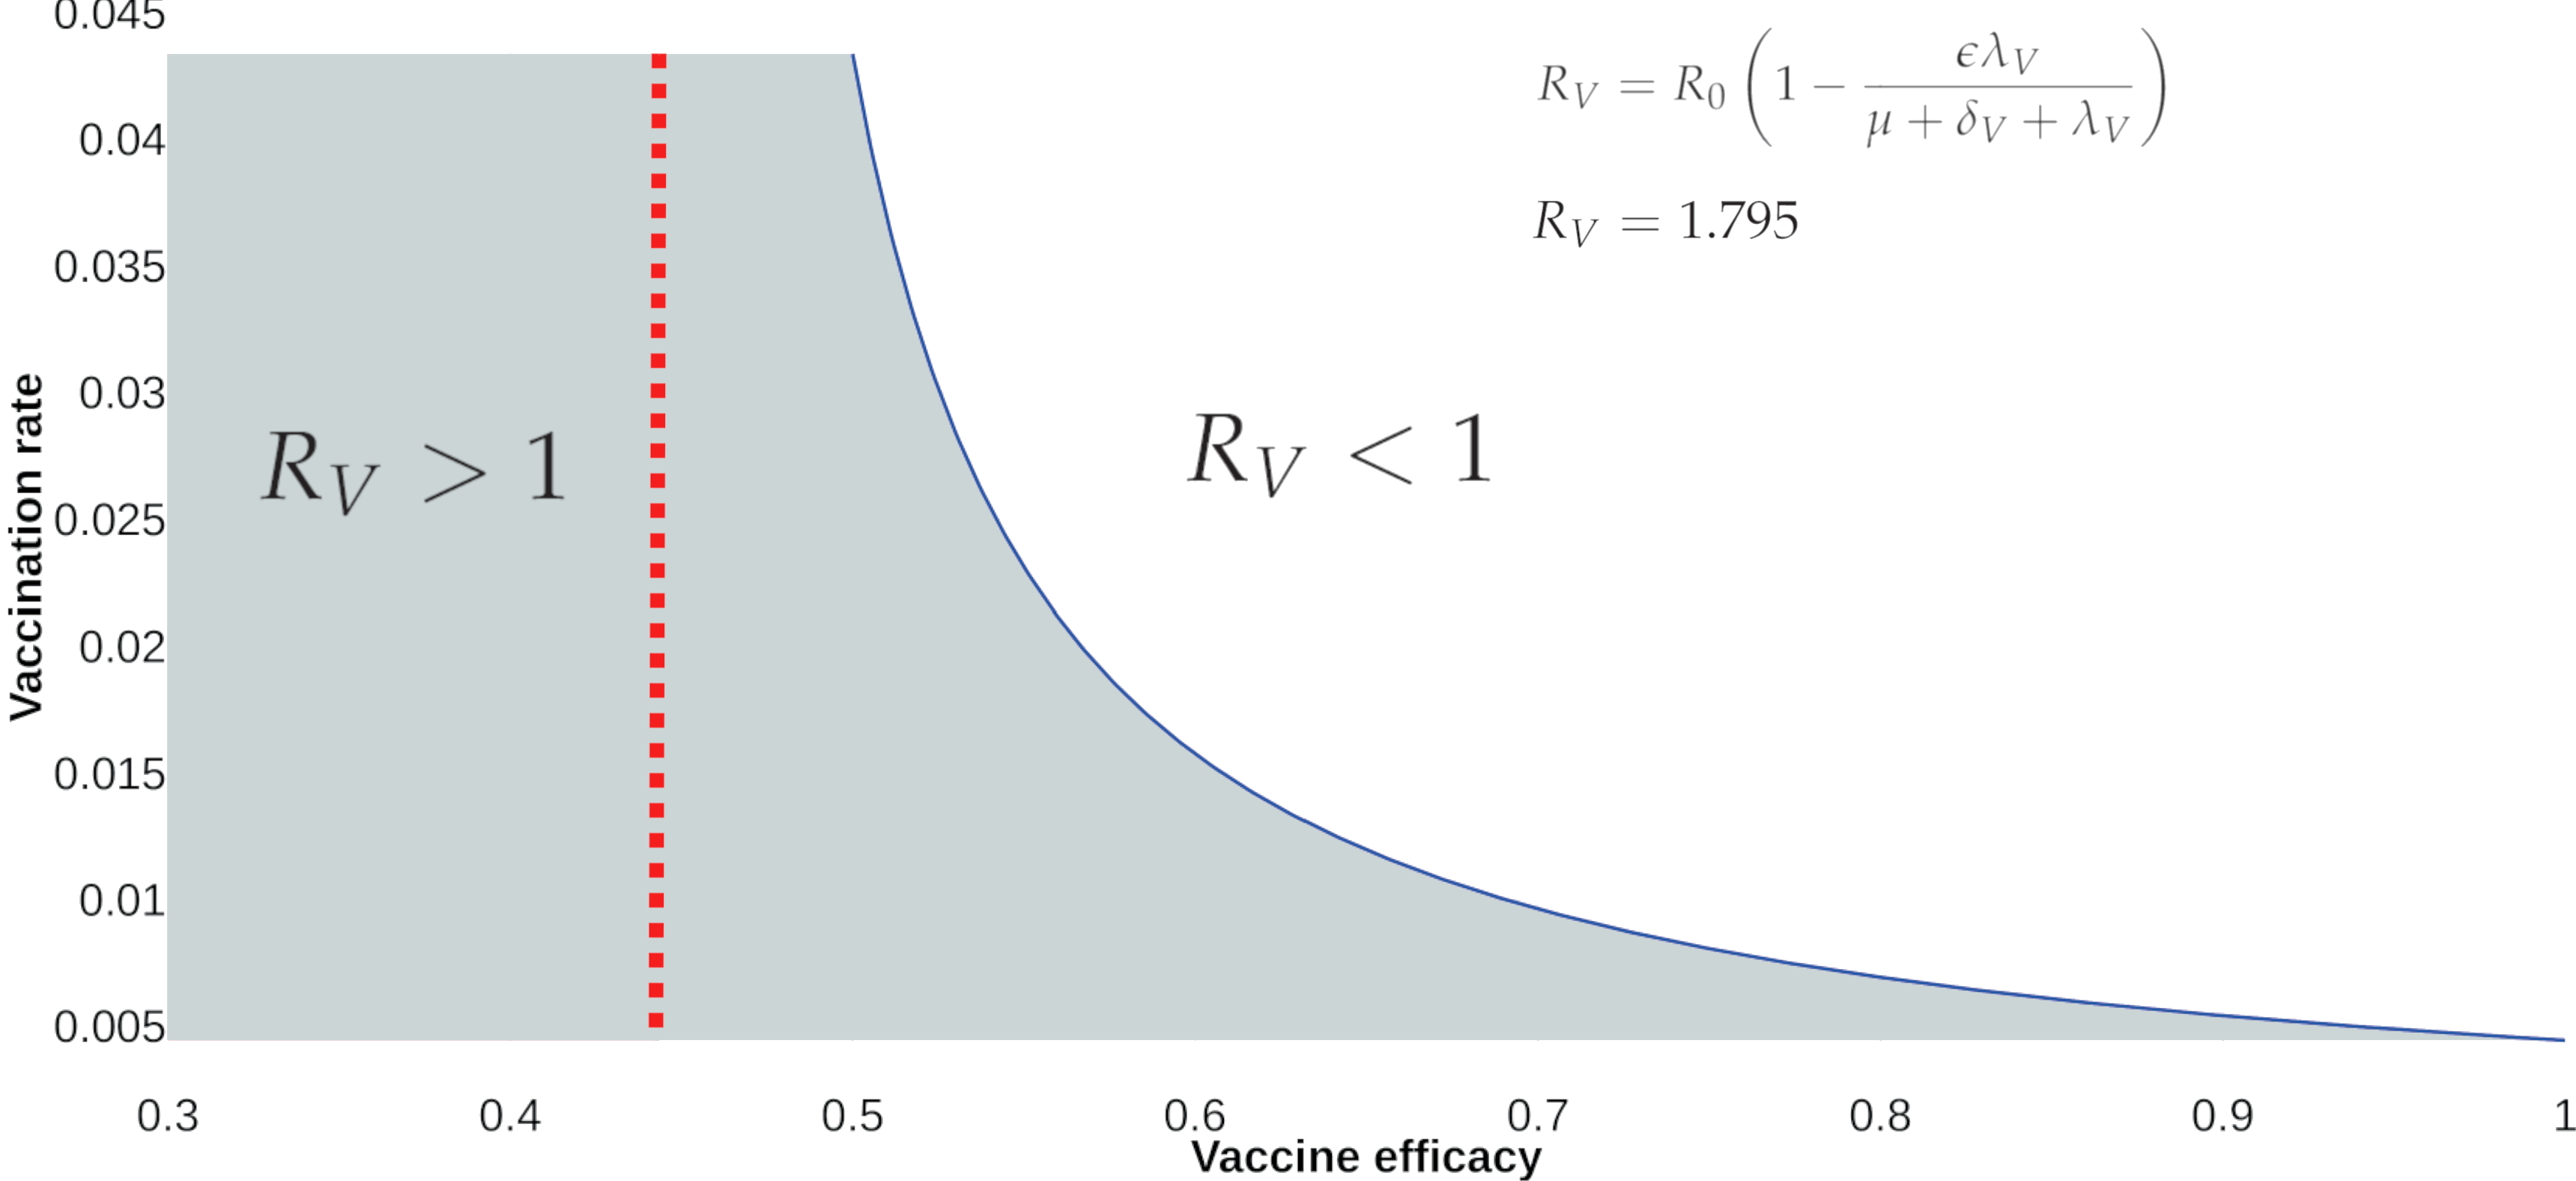
\includegraphics[scale=.875,%
            keepaspectratio]{assets/RvAnimation//r_zero_vac_efficiency03.png}
        }
        \only<4>{
            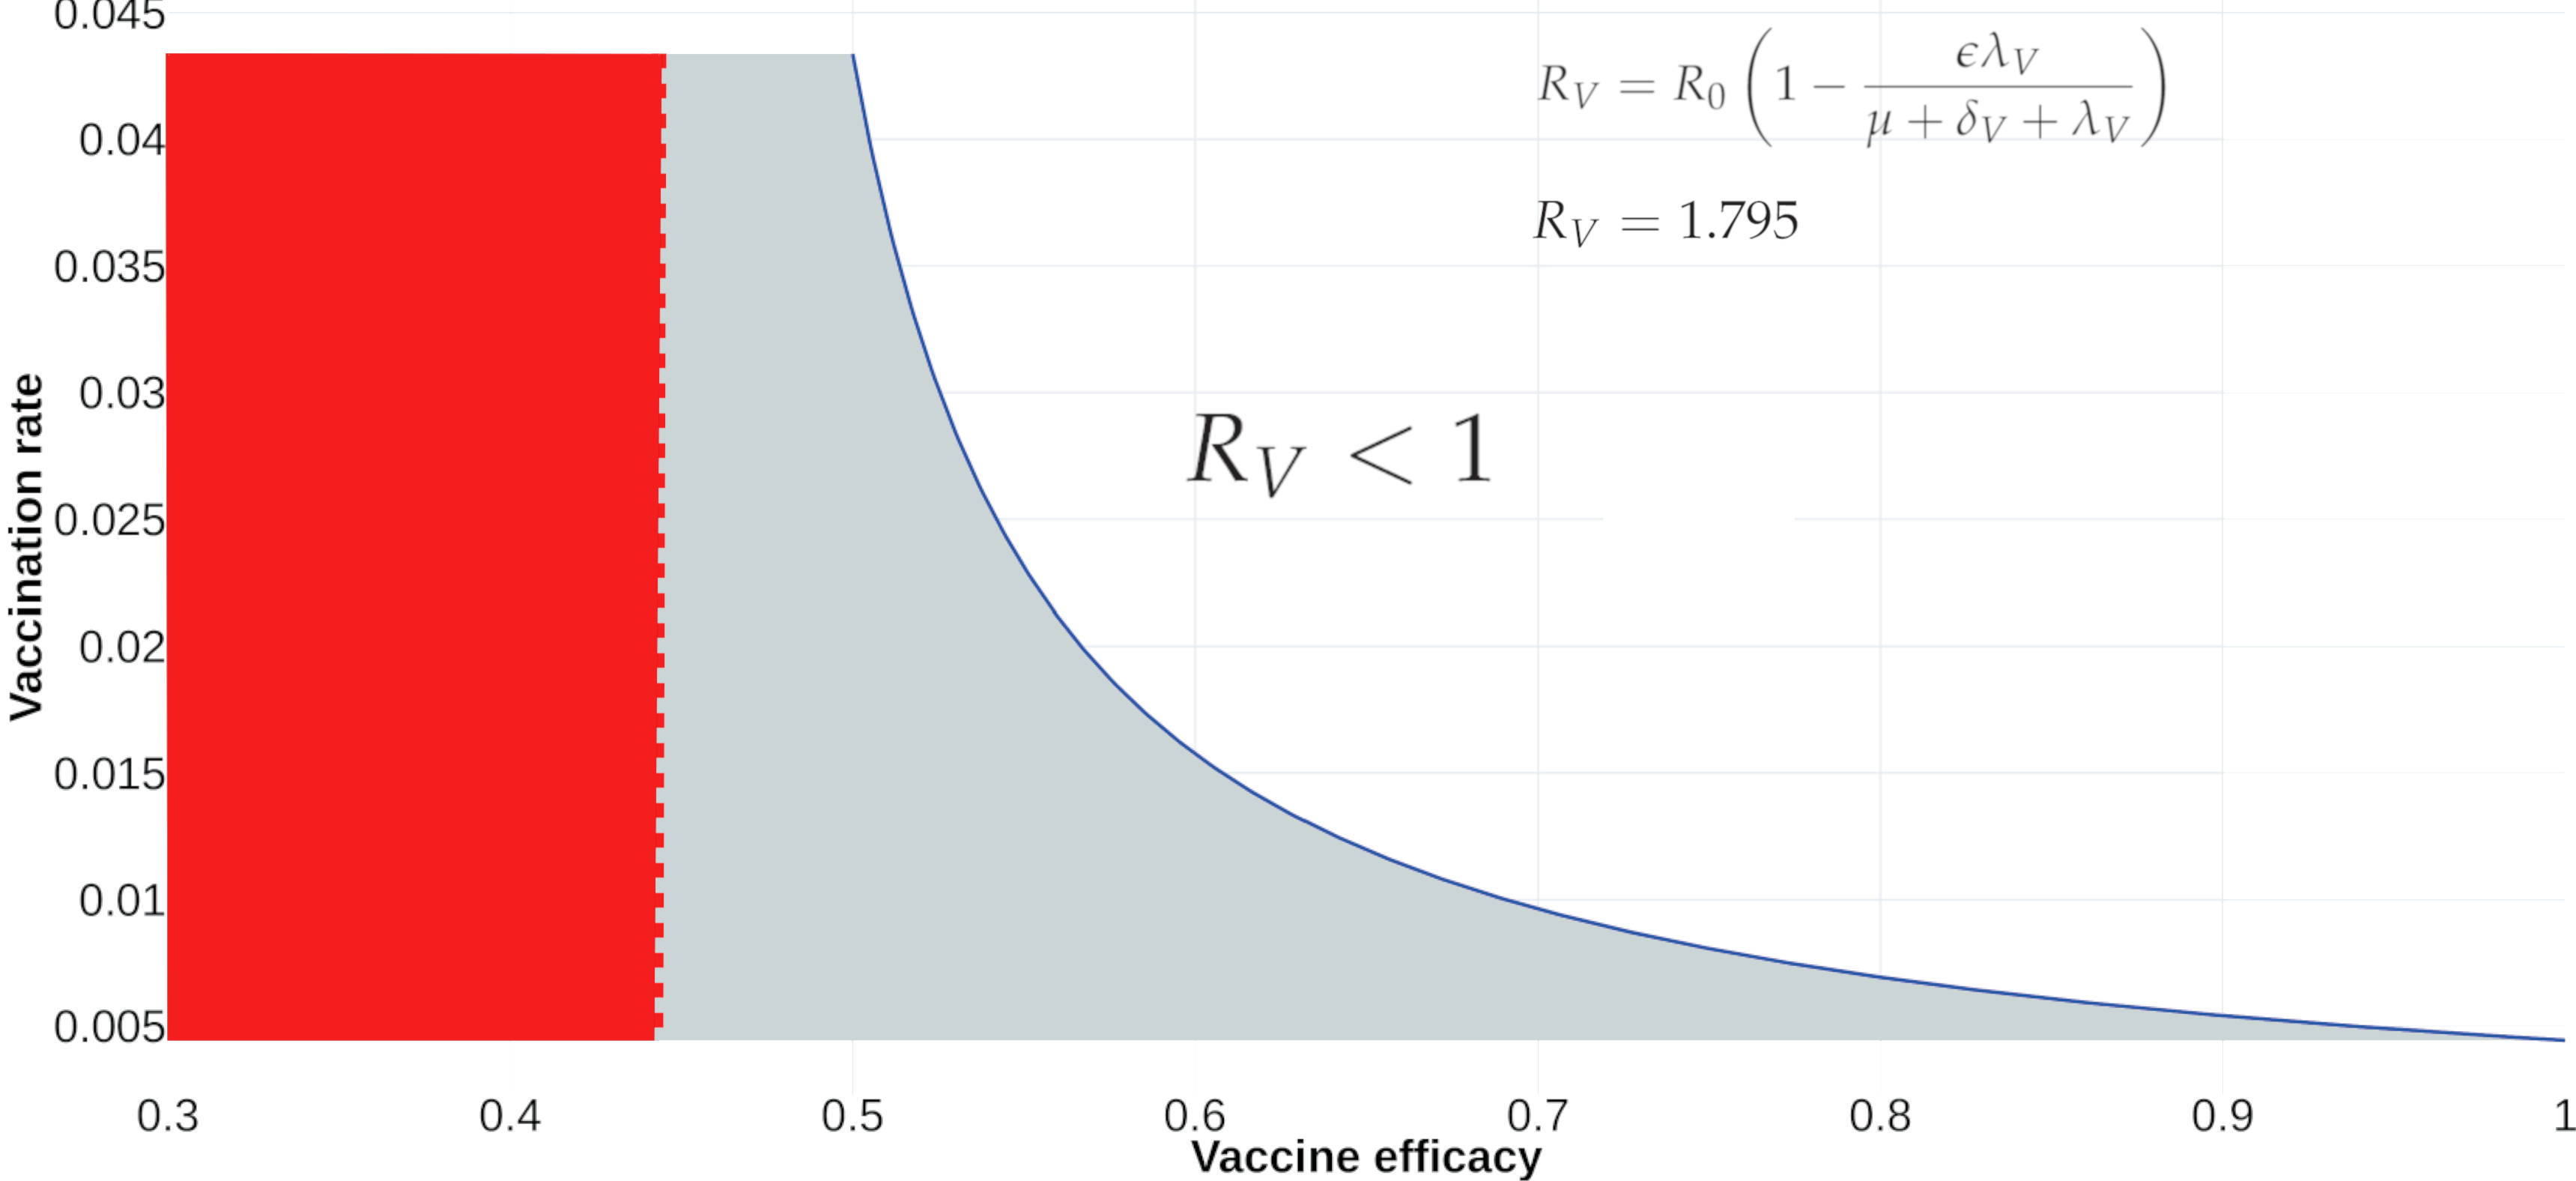
\includegraphics[scale=.875,%
            keepaspectratio]{assets/RvAnimation//r_zero_vac_efficiency04.png}
        }
        \only<5>{
            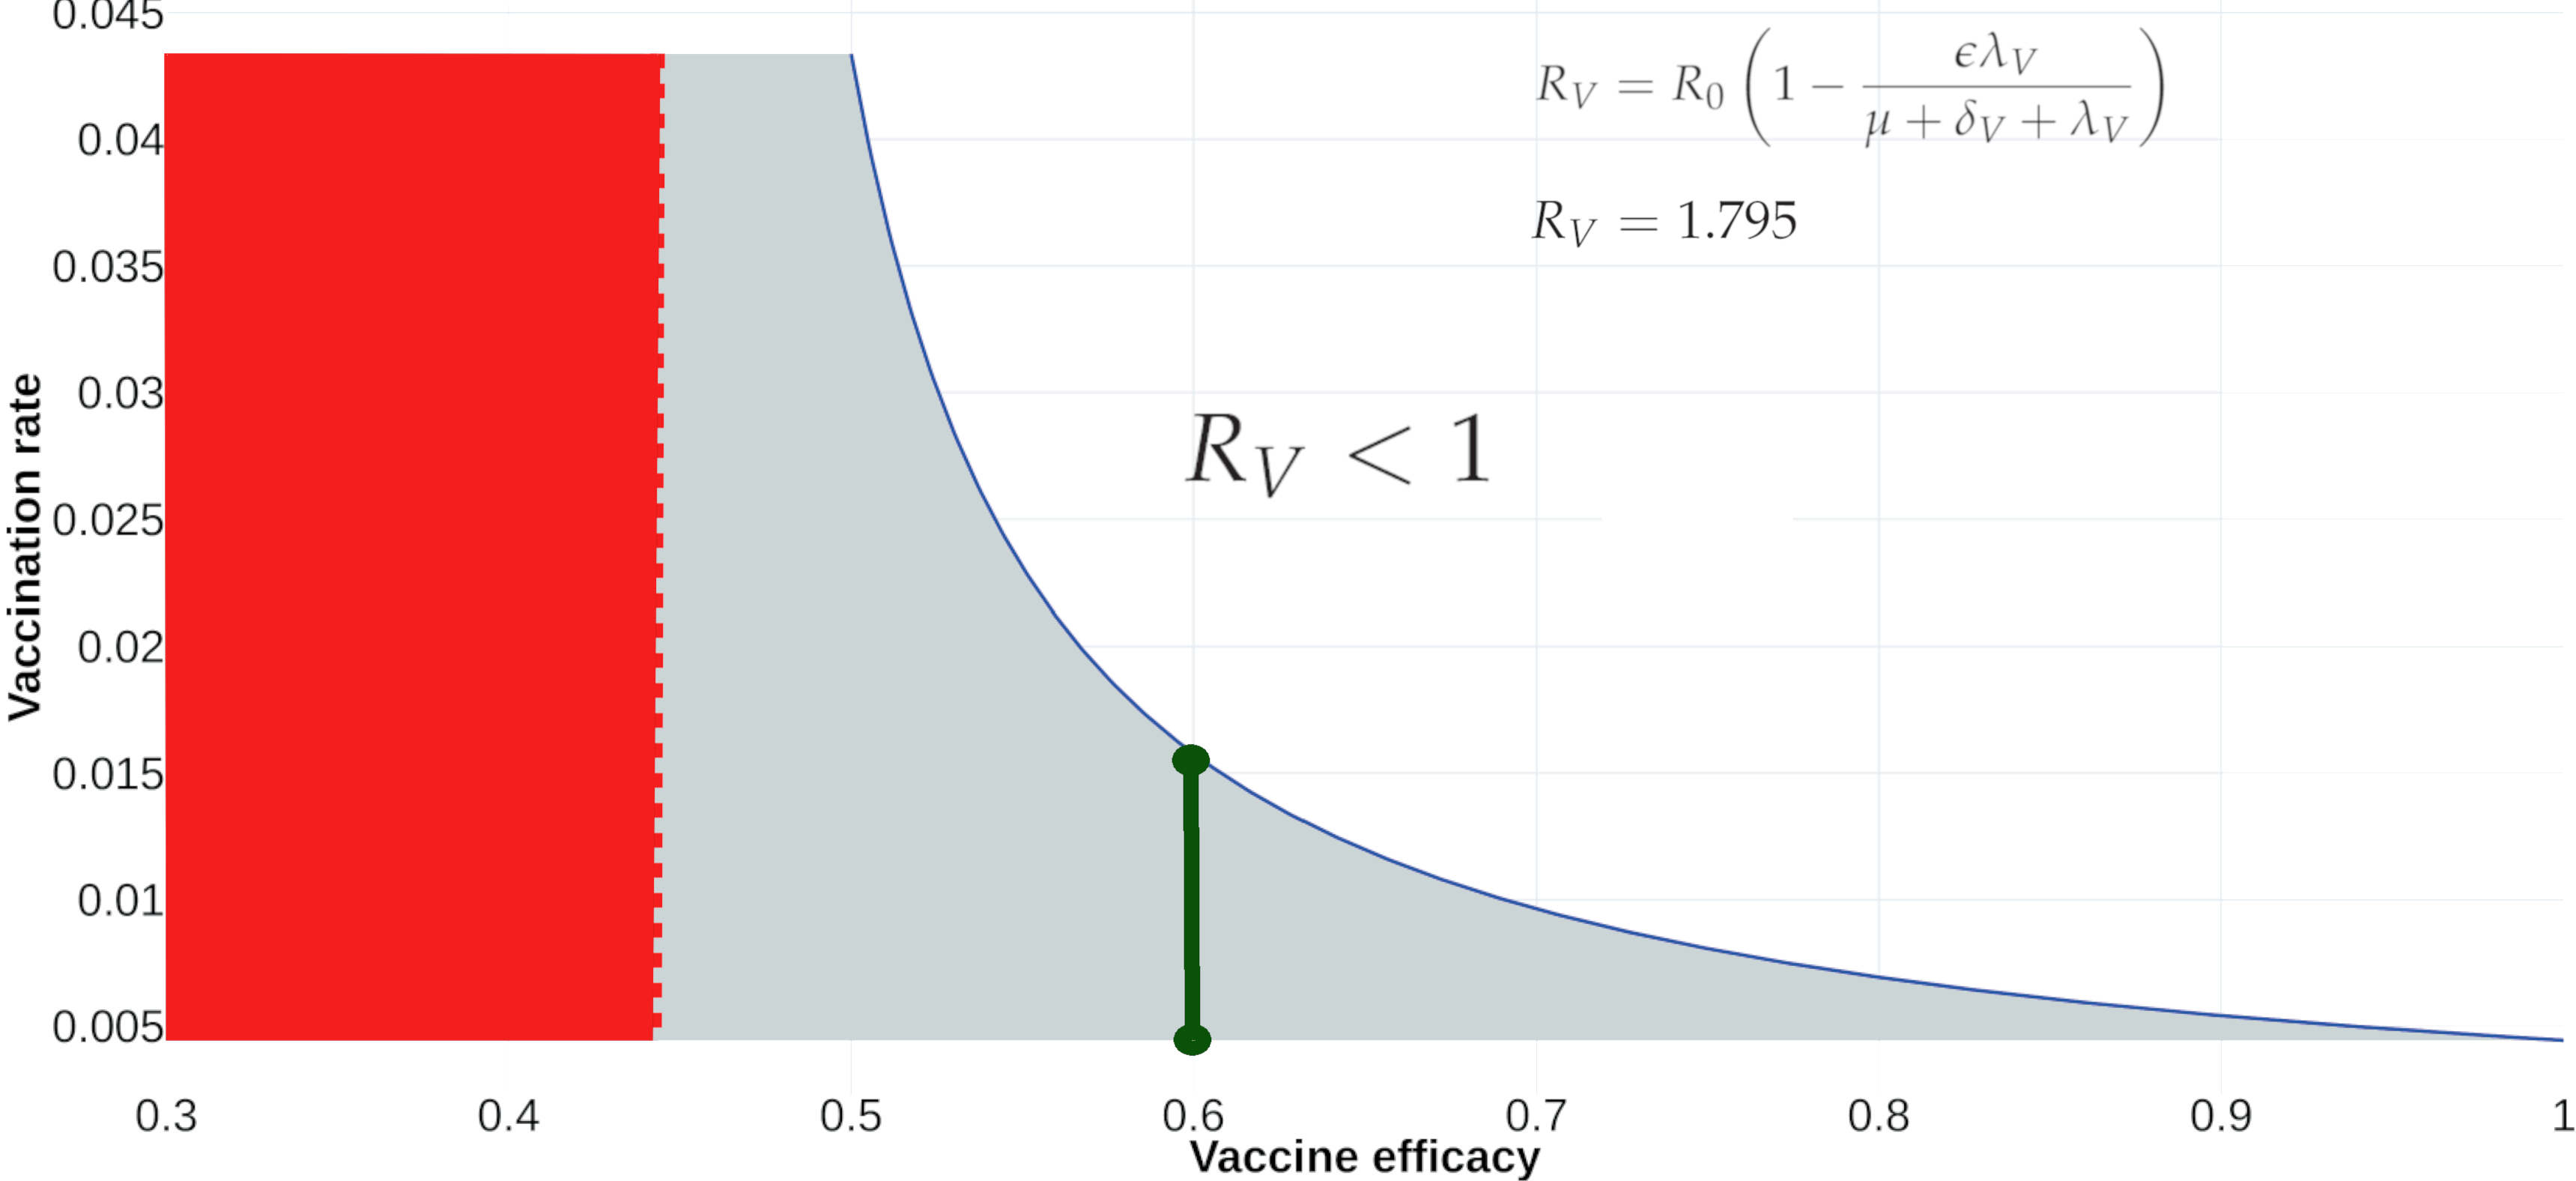
\includegraphics[scale=.875,%
            keepaspectratio]{assets/RvAnimation//r_zero_vac_efficiency05.png}
        }
        \only<6>{
            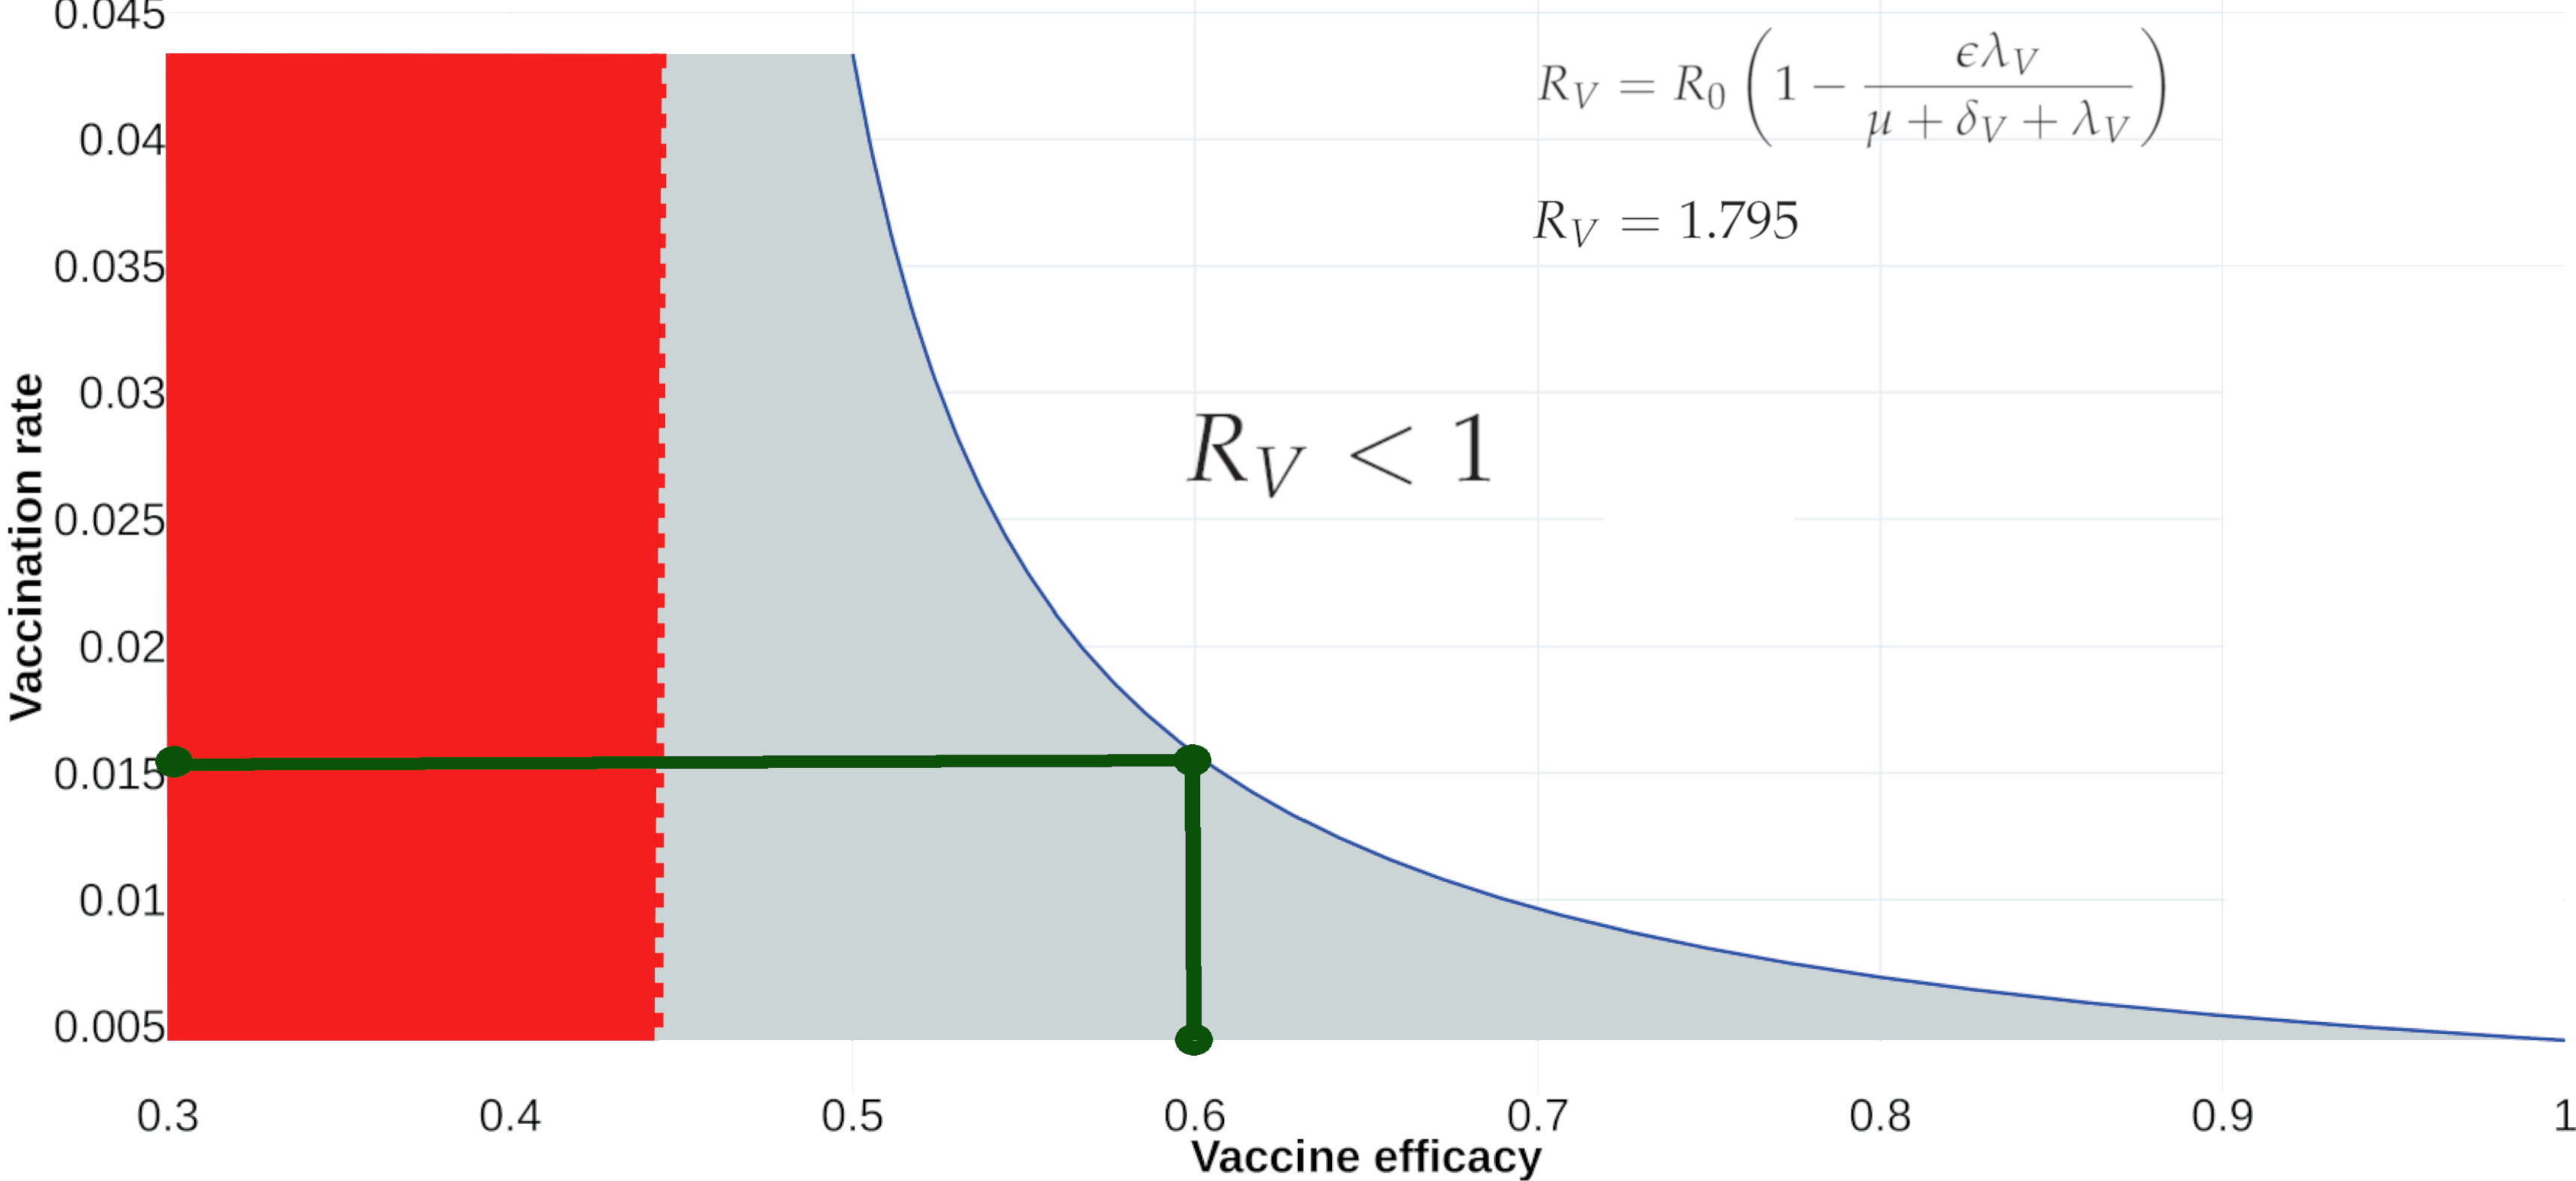
\includegraphics[scale=.875,%
            keepaspectratio]{assets/RvAnimation/r_zero_vac_efficiency06.png}
        }

    \end{textblock*}
%     \begin{textblock*}{120mm}(0mm, 10mm)
%         \only<7>{
%             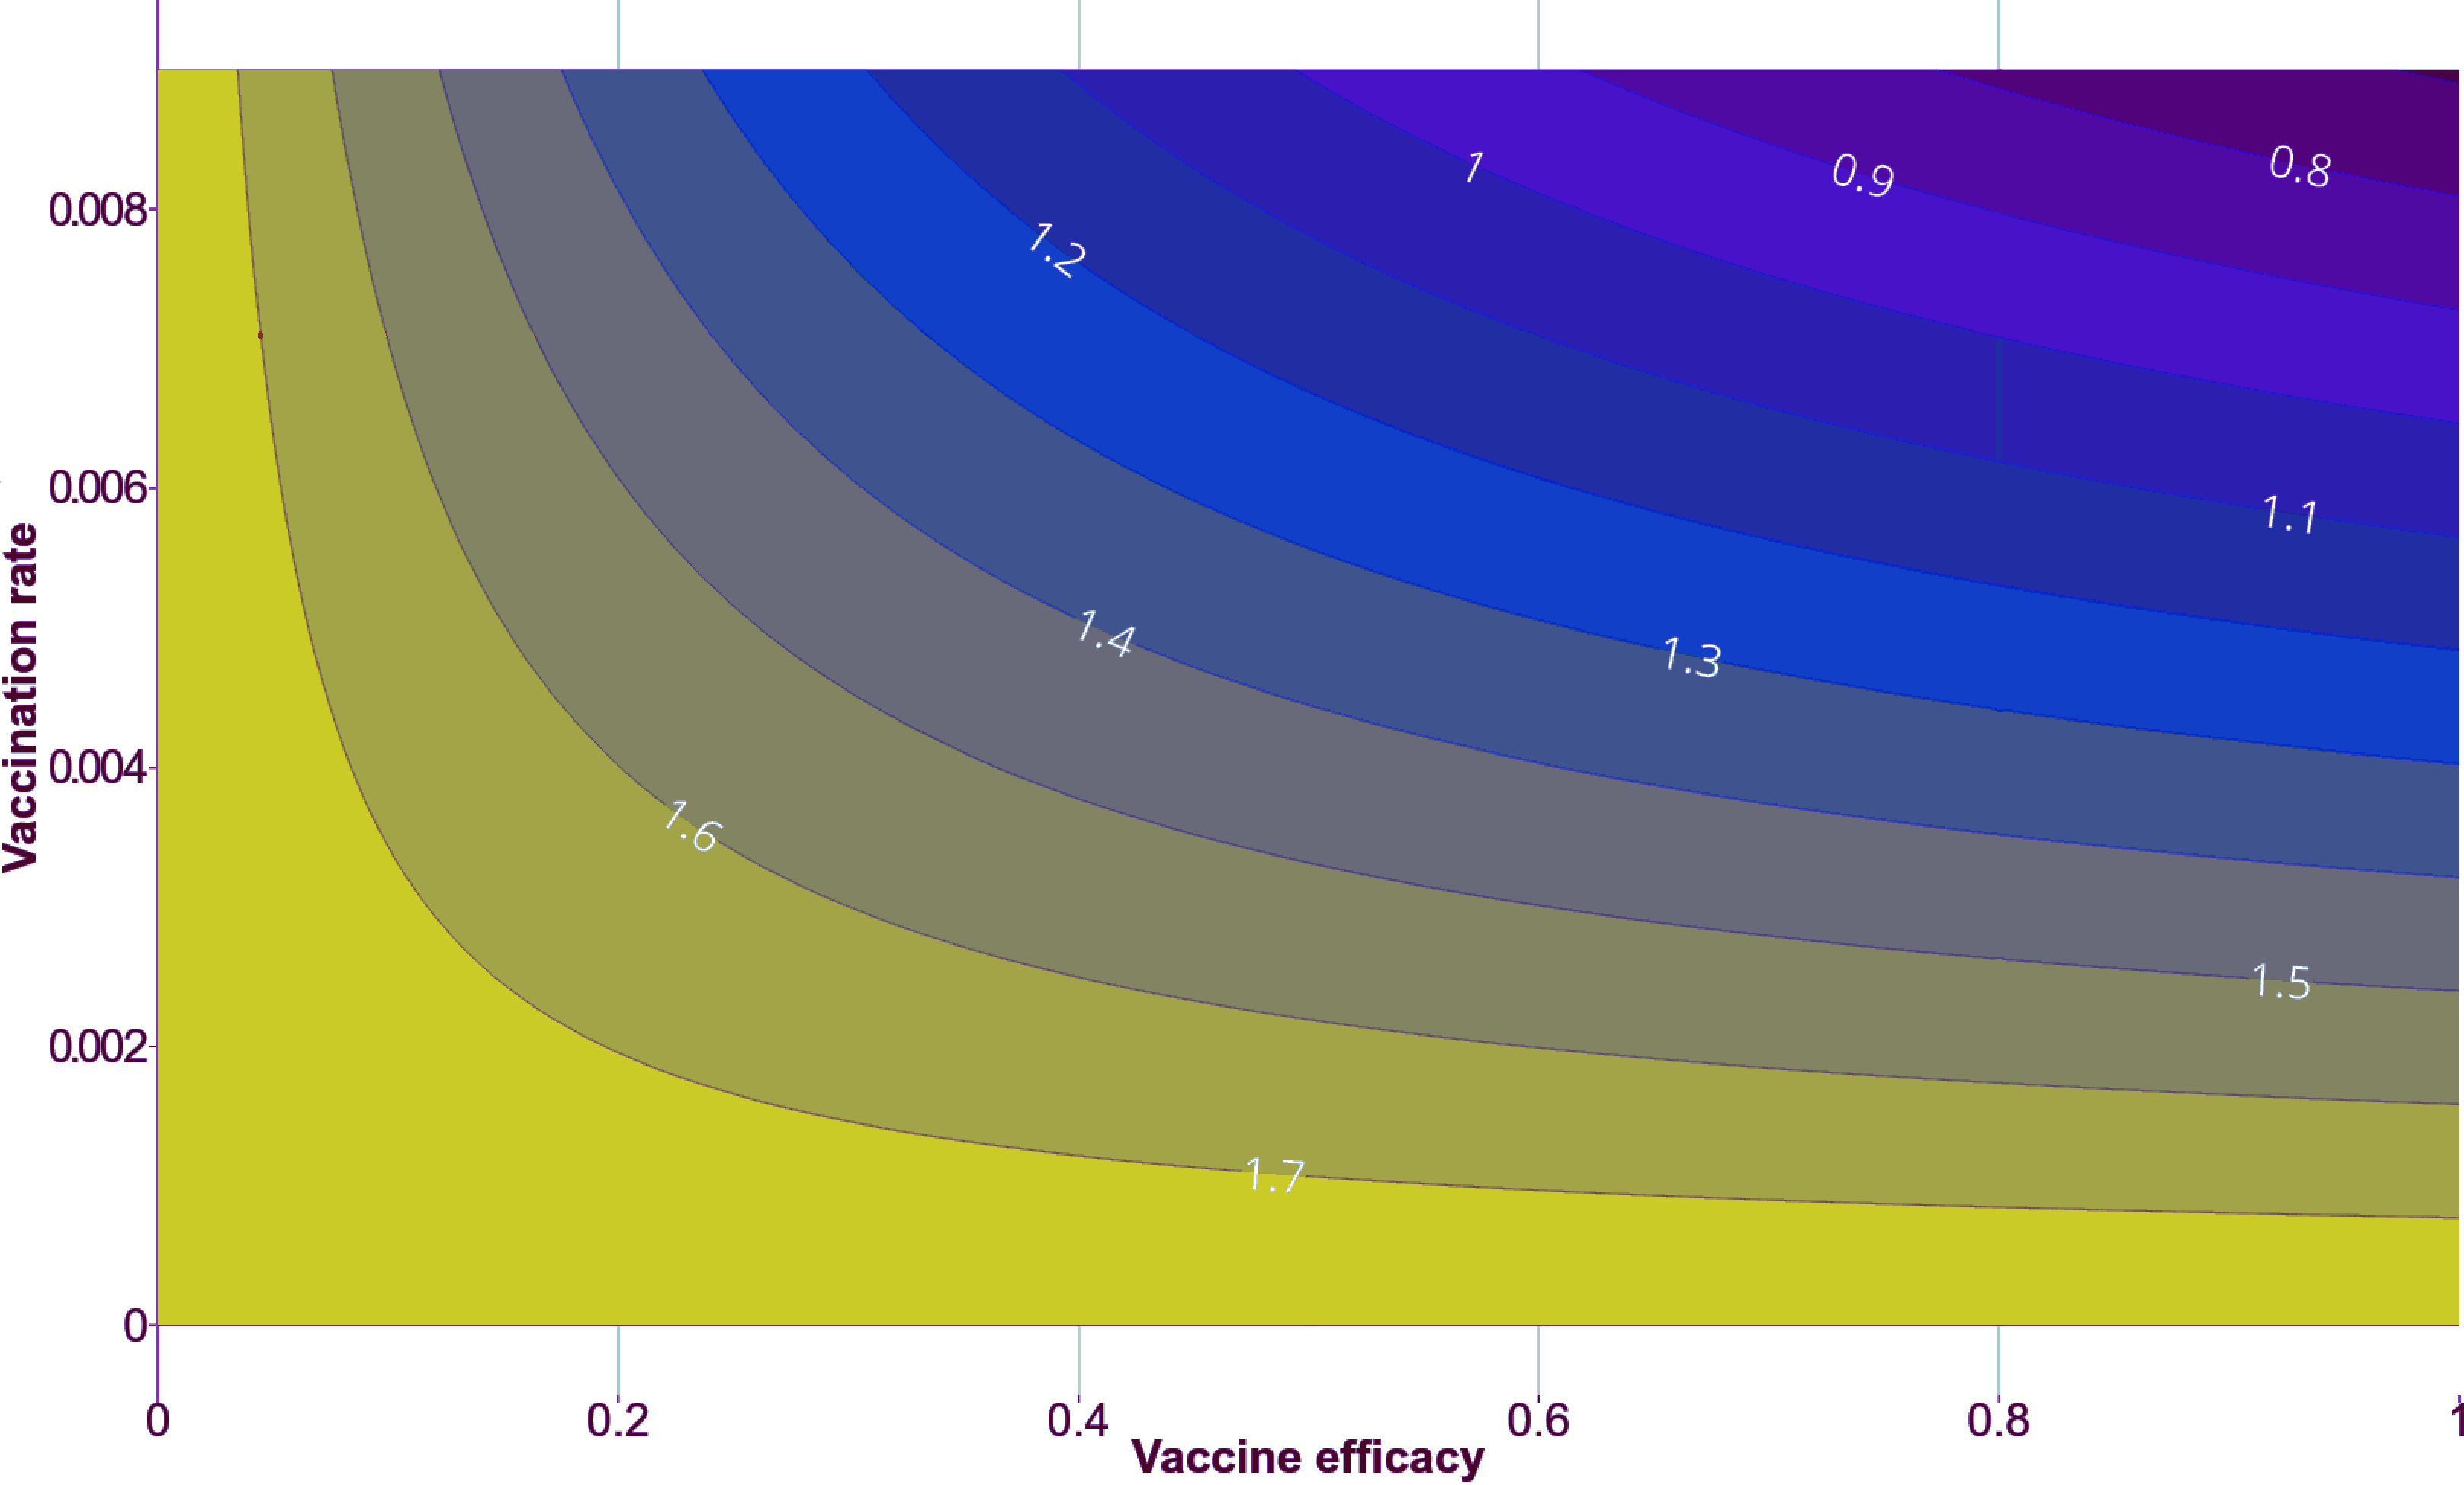
\includegraphics[scale=.65,%
%             keepaspectratio]{assets/RvAnimation/r_zero_vac_level_plots01.png}
%         }
%         \only<8>{
%             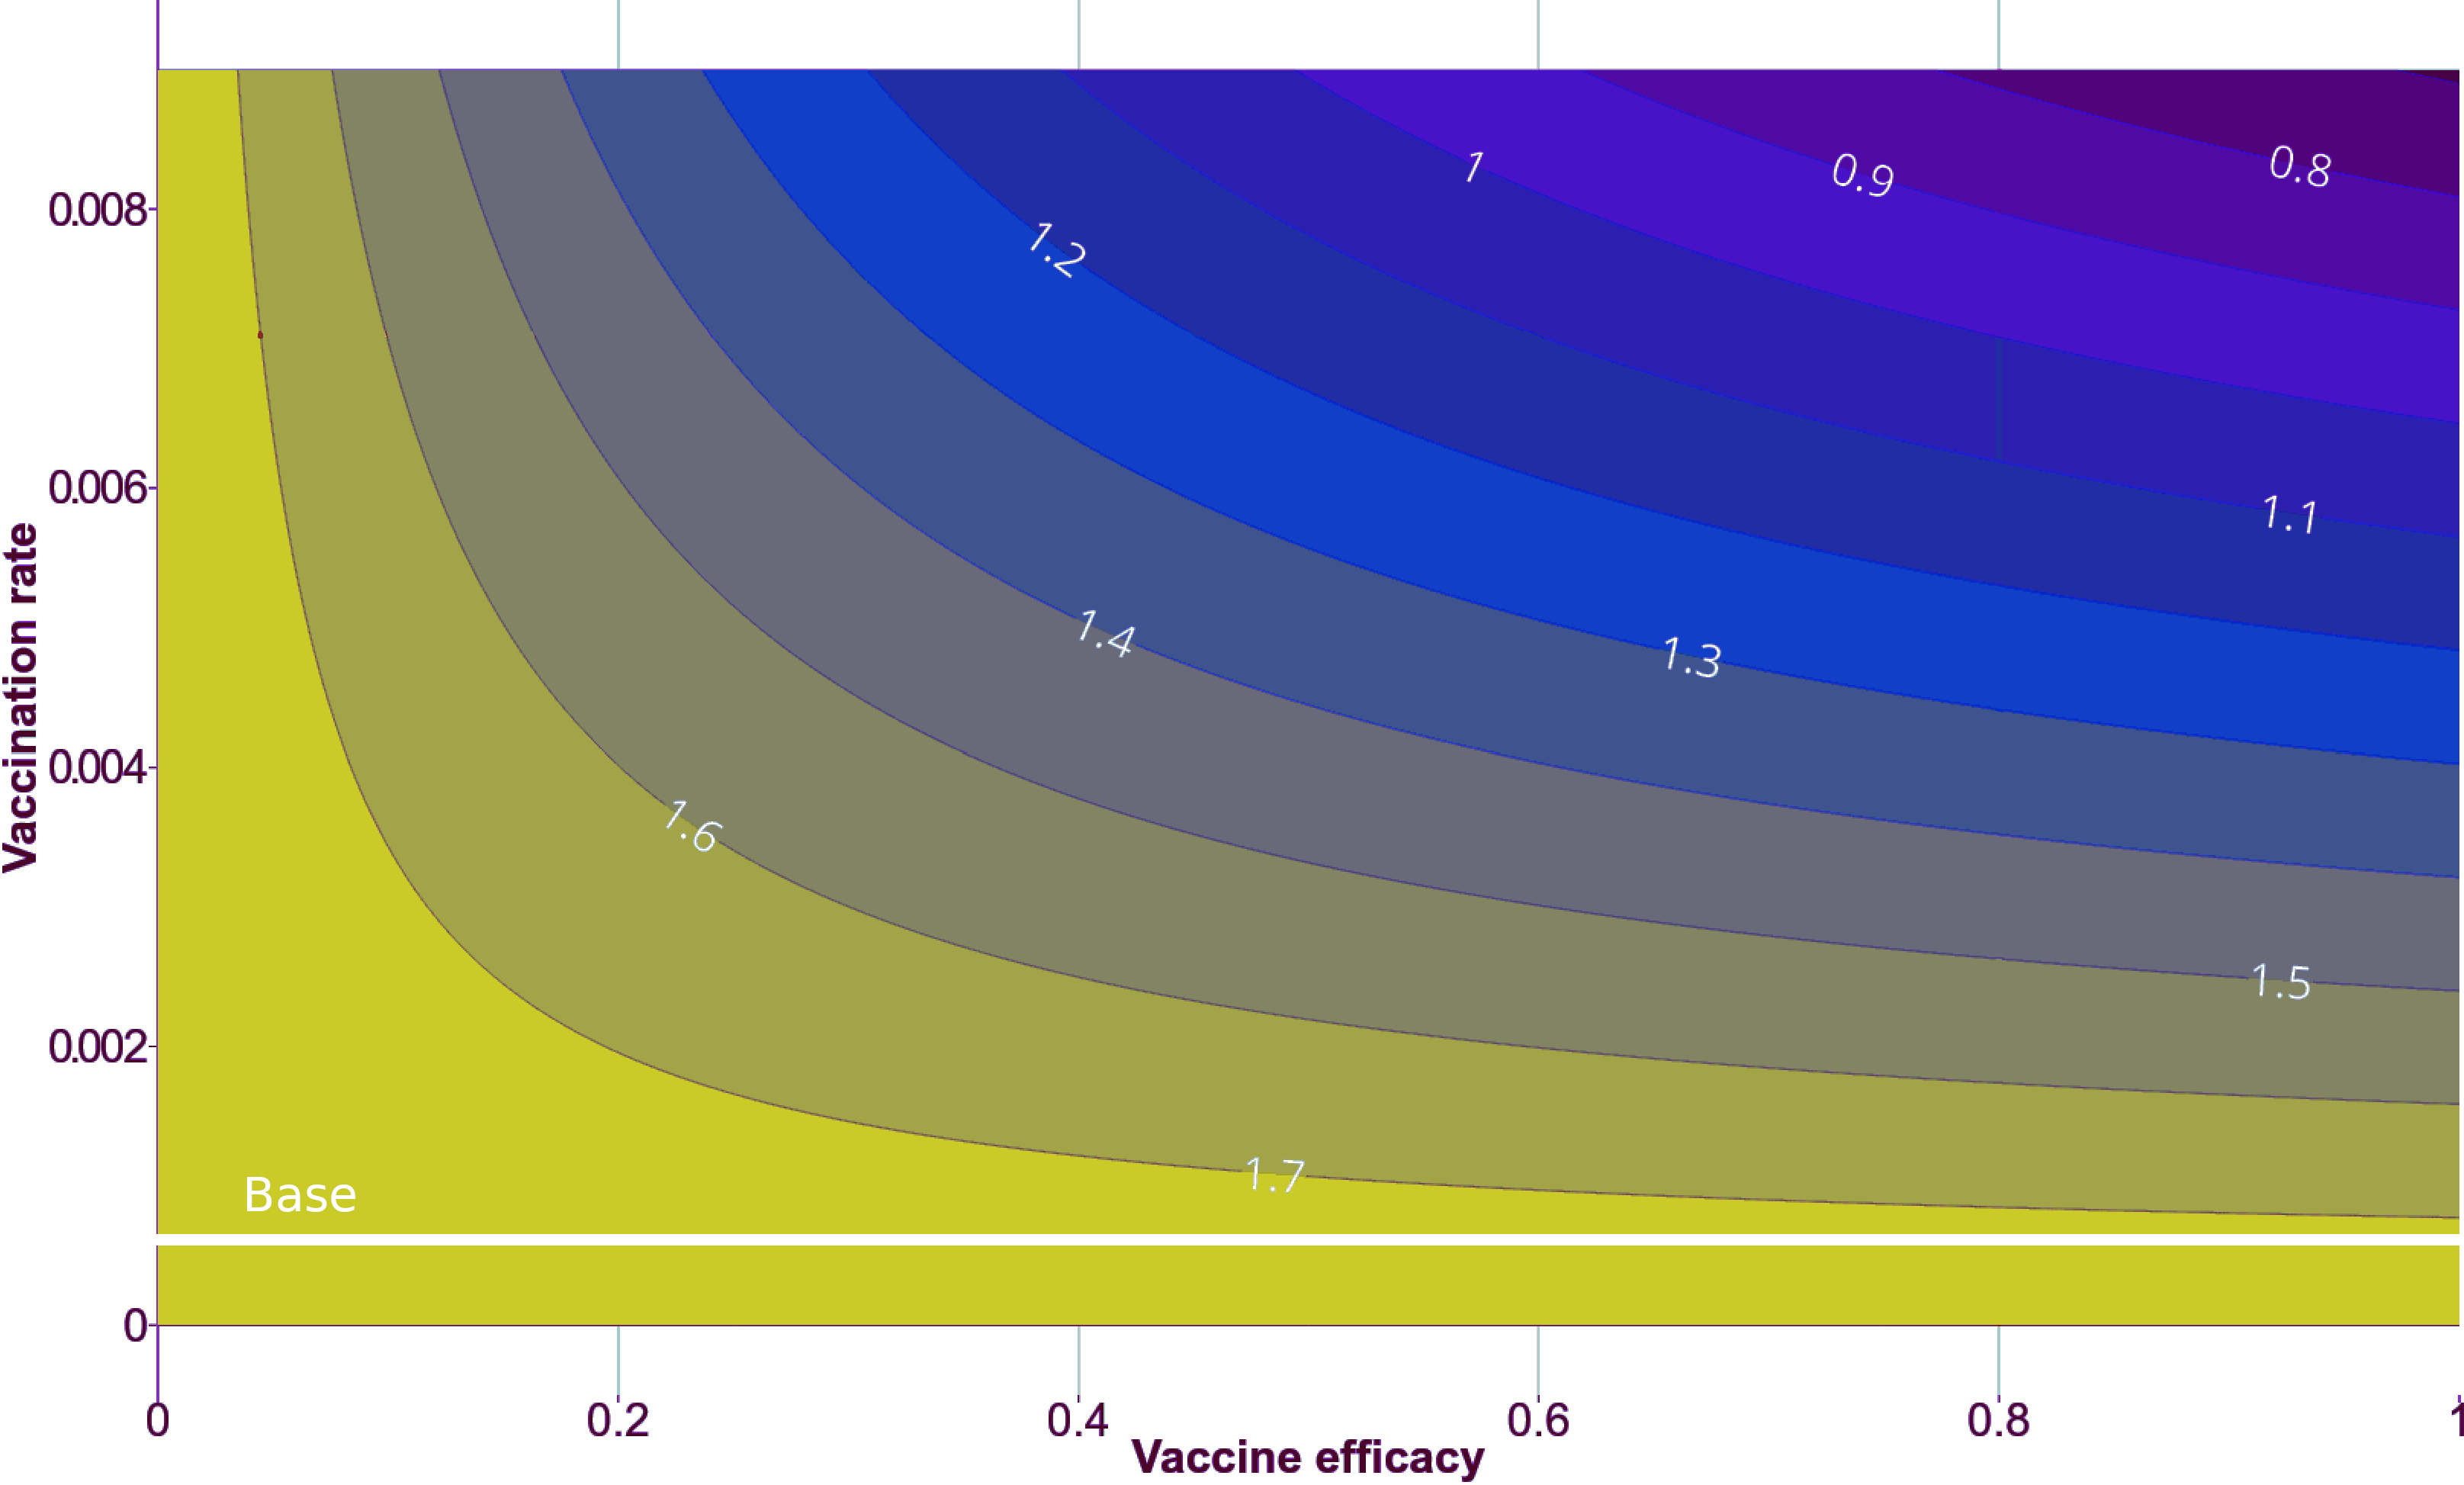
\includegraphics[scale=.65,%
%              keepaspectratio]{assets/RvAnimation/r_zero_vac_level_plots02.png}
%         }
%         \only<9>{
%             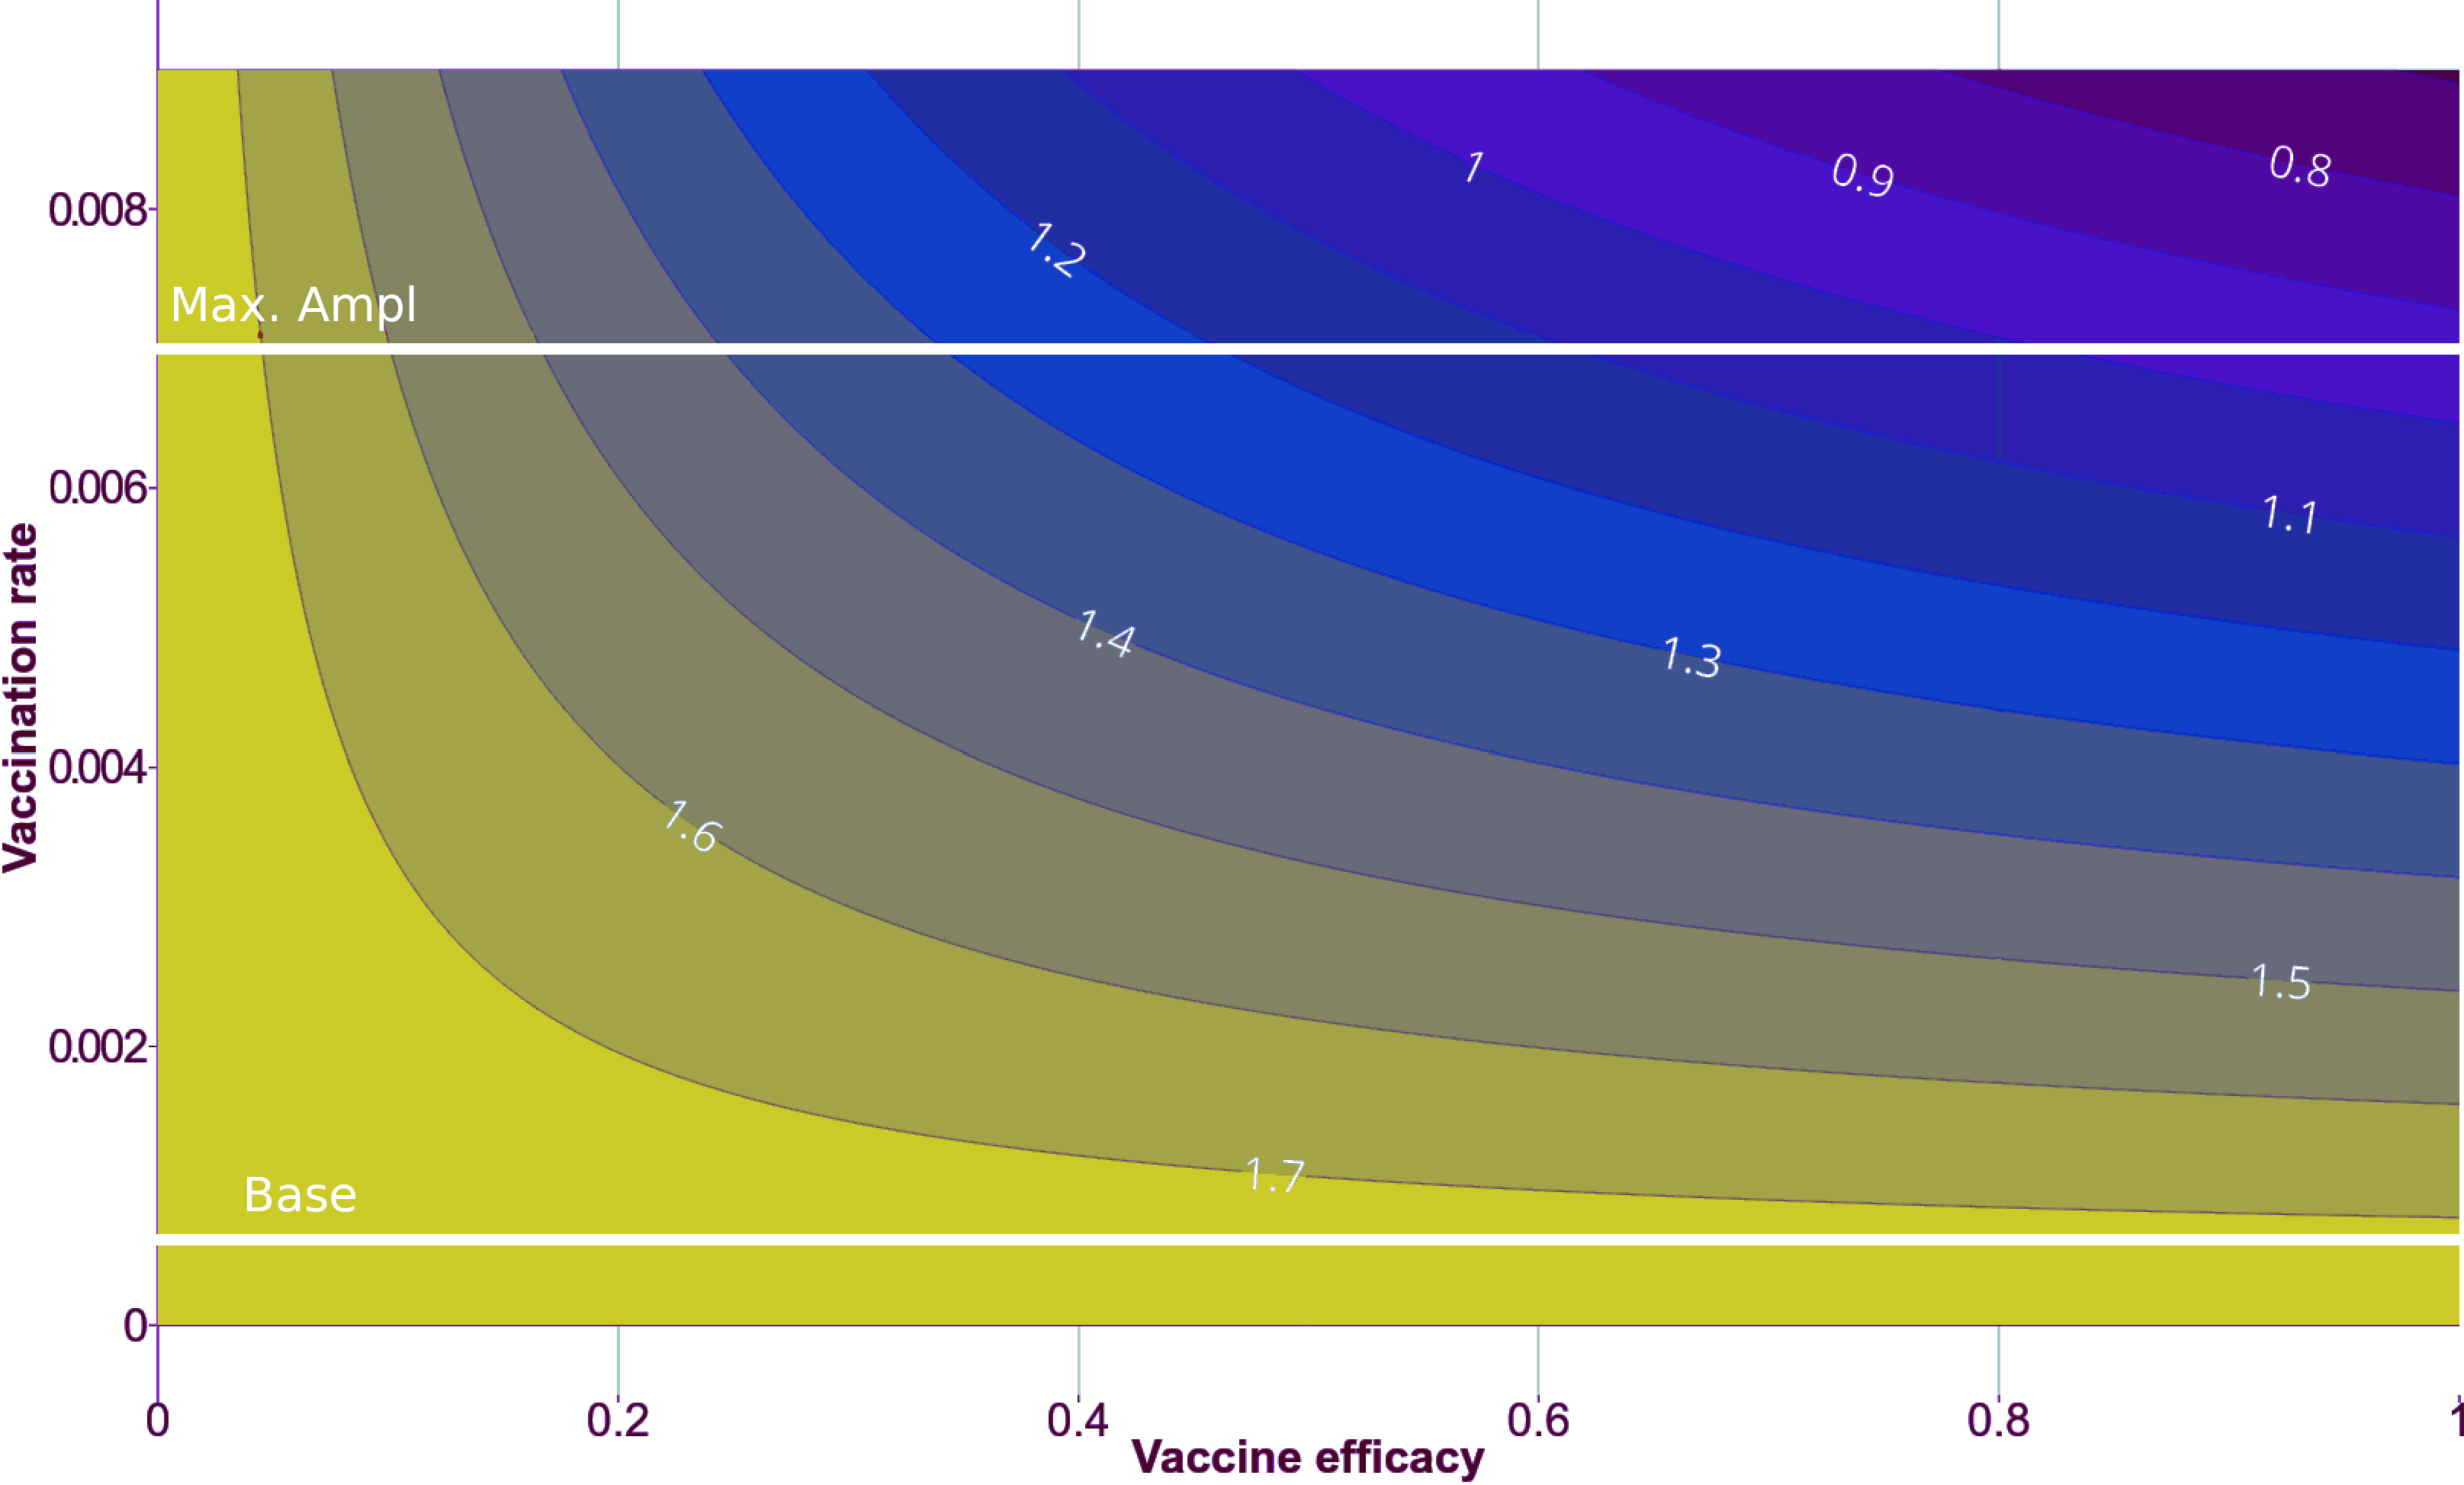
\includegraphics[scale=.65,%
%              keepaspectratio]{assets/RvAnimation/r_zero_vac_level_plots03.png}
%         }
%         \only<10>{
%             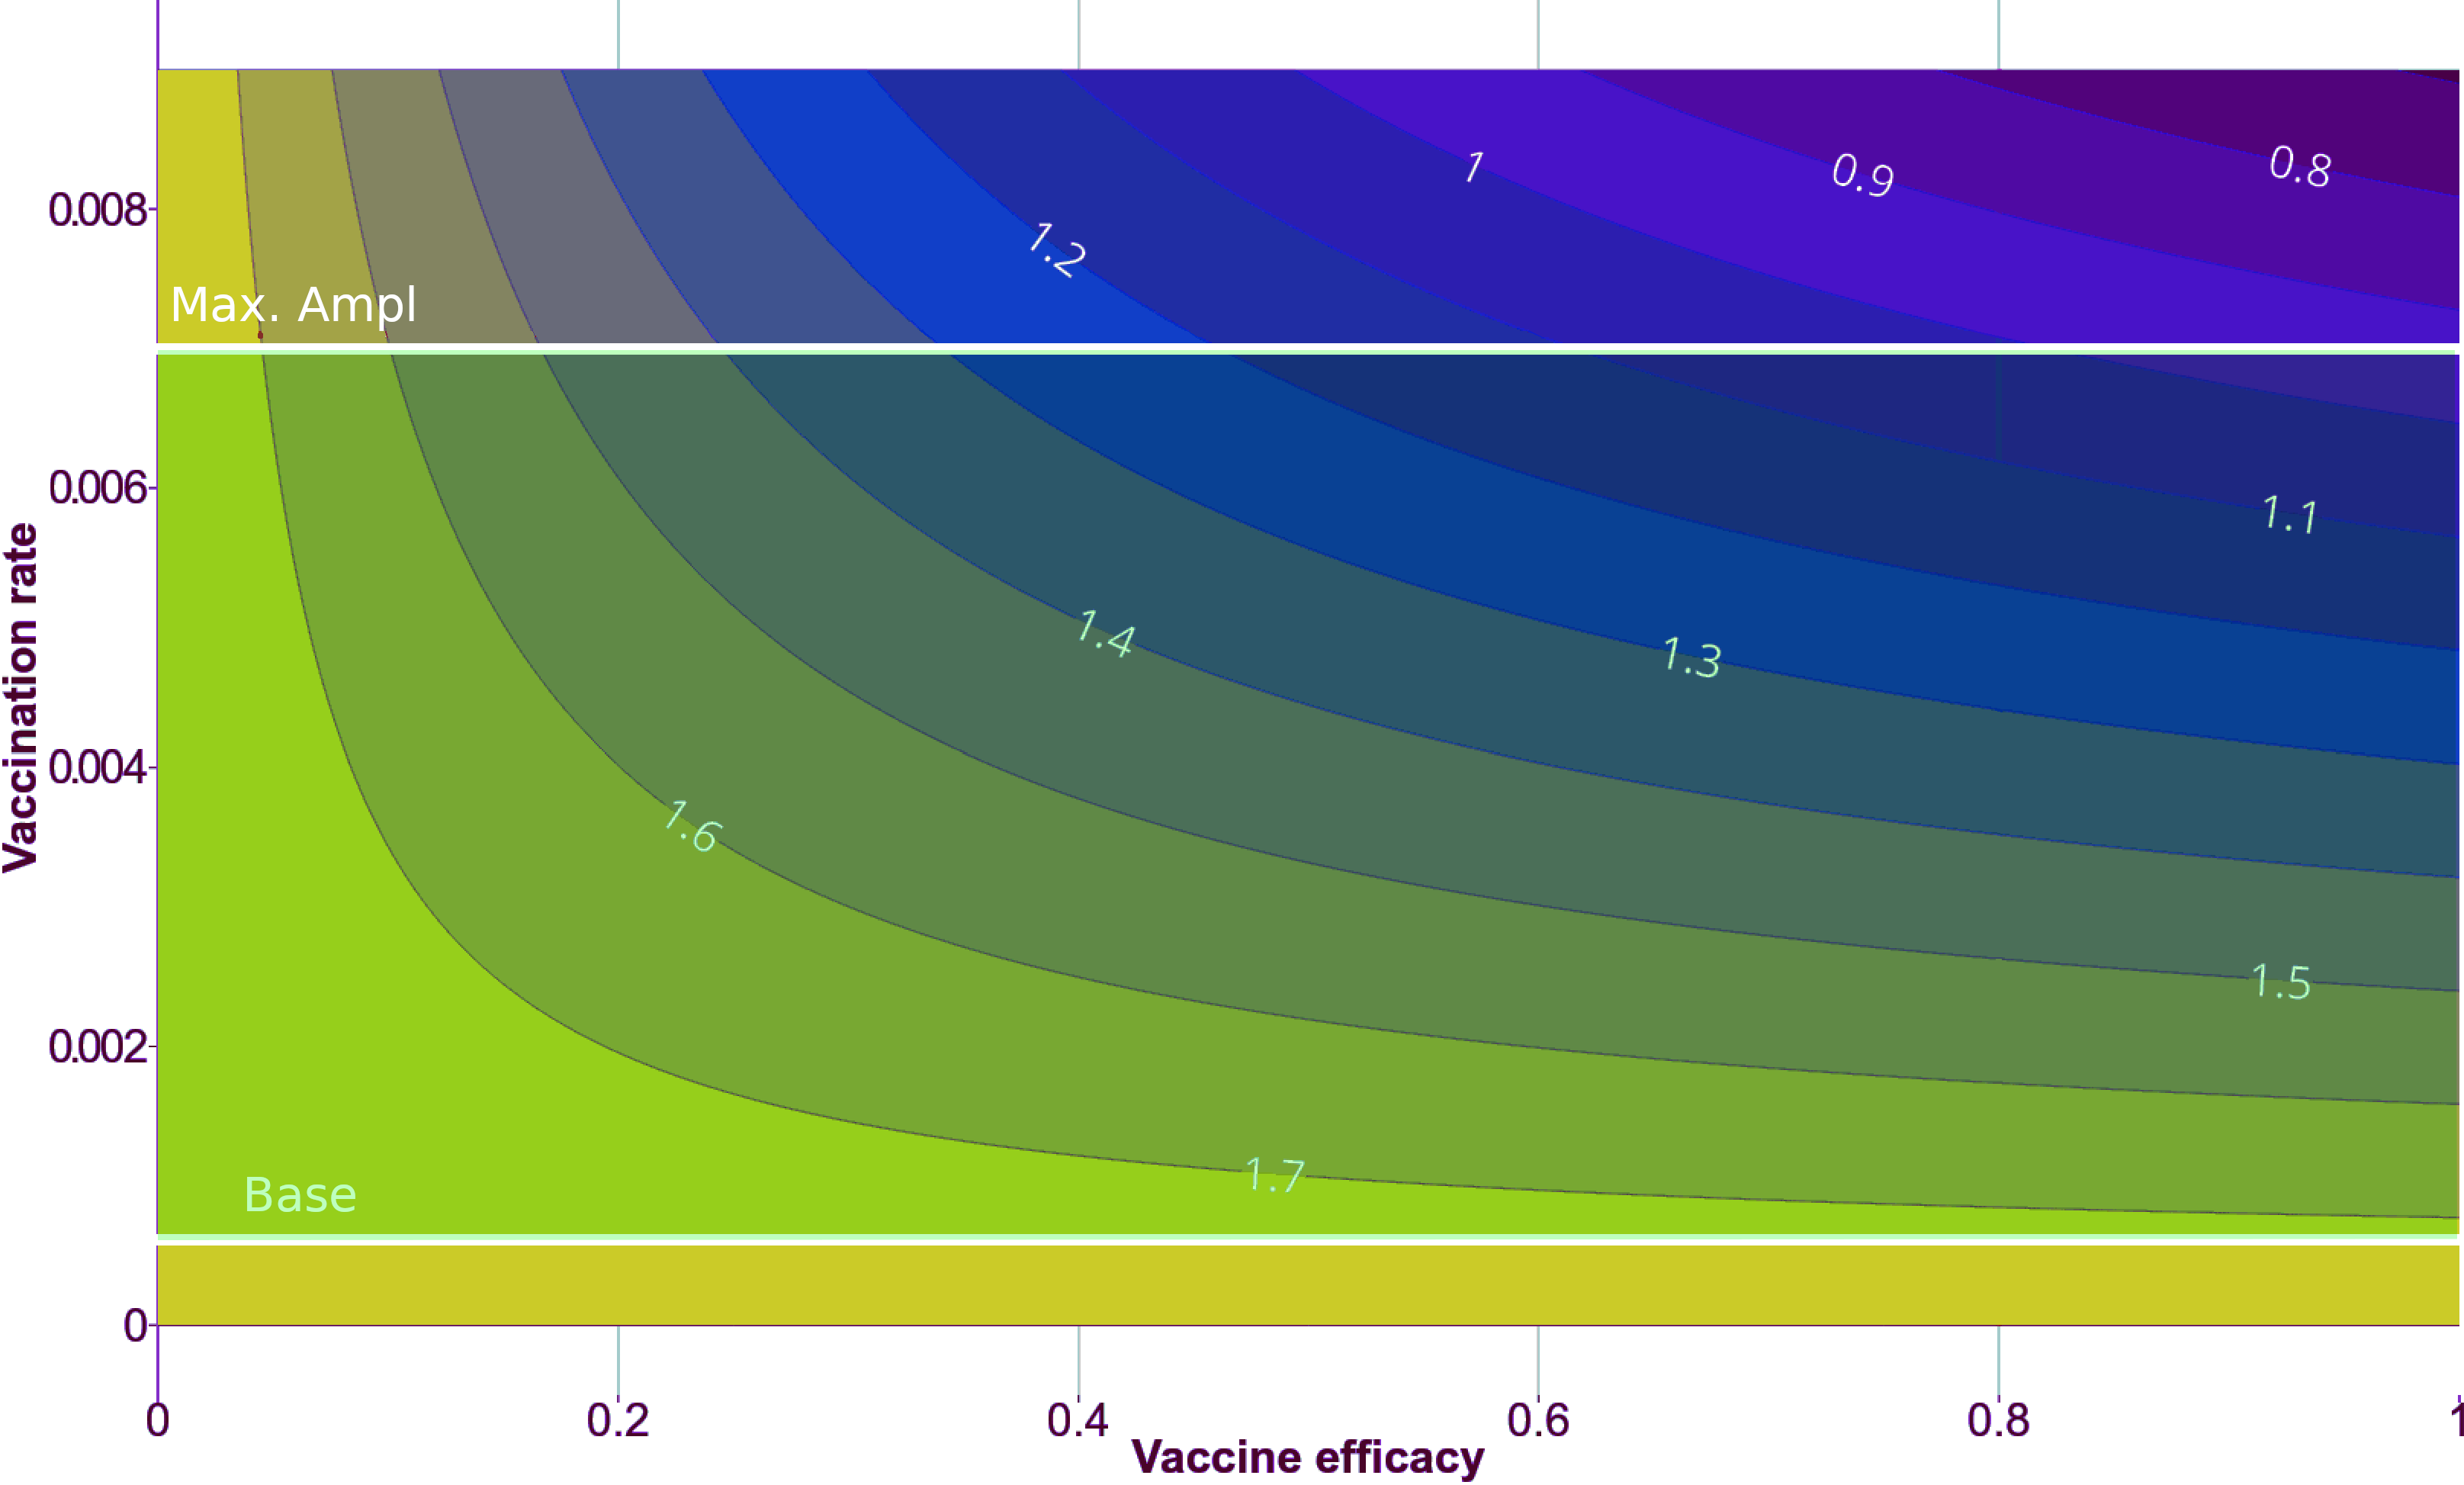
\includegraphics[scale=.65,%
%              keepaspectratio]{assets/RvAnimation/r_zero_vac_level_plots04.png}
%         }
%         \only<11>{
%             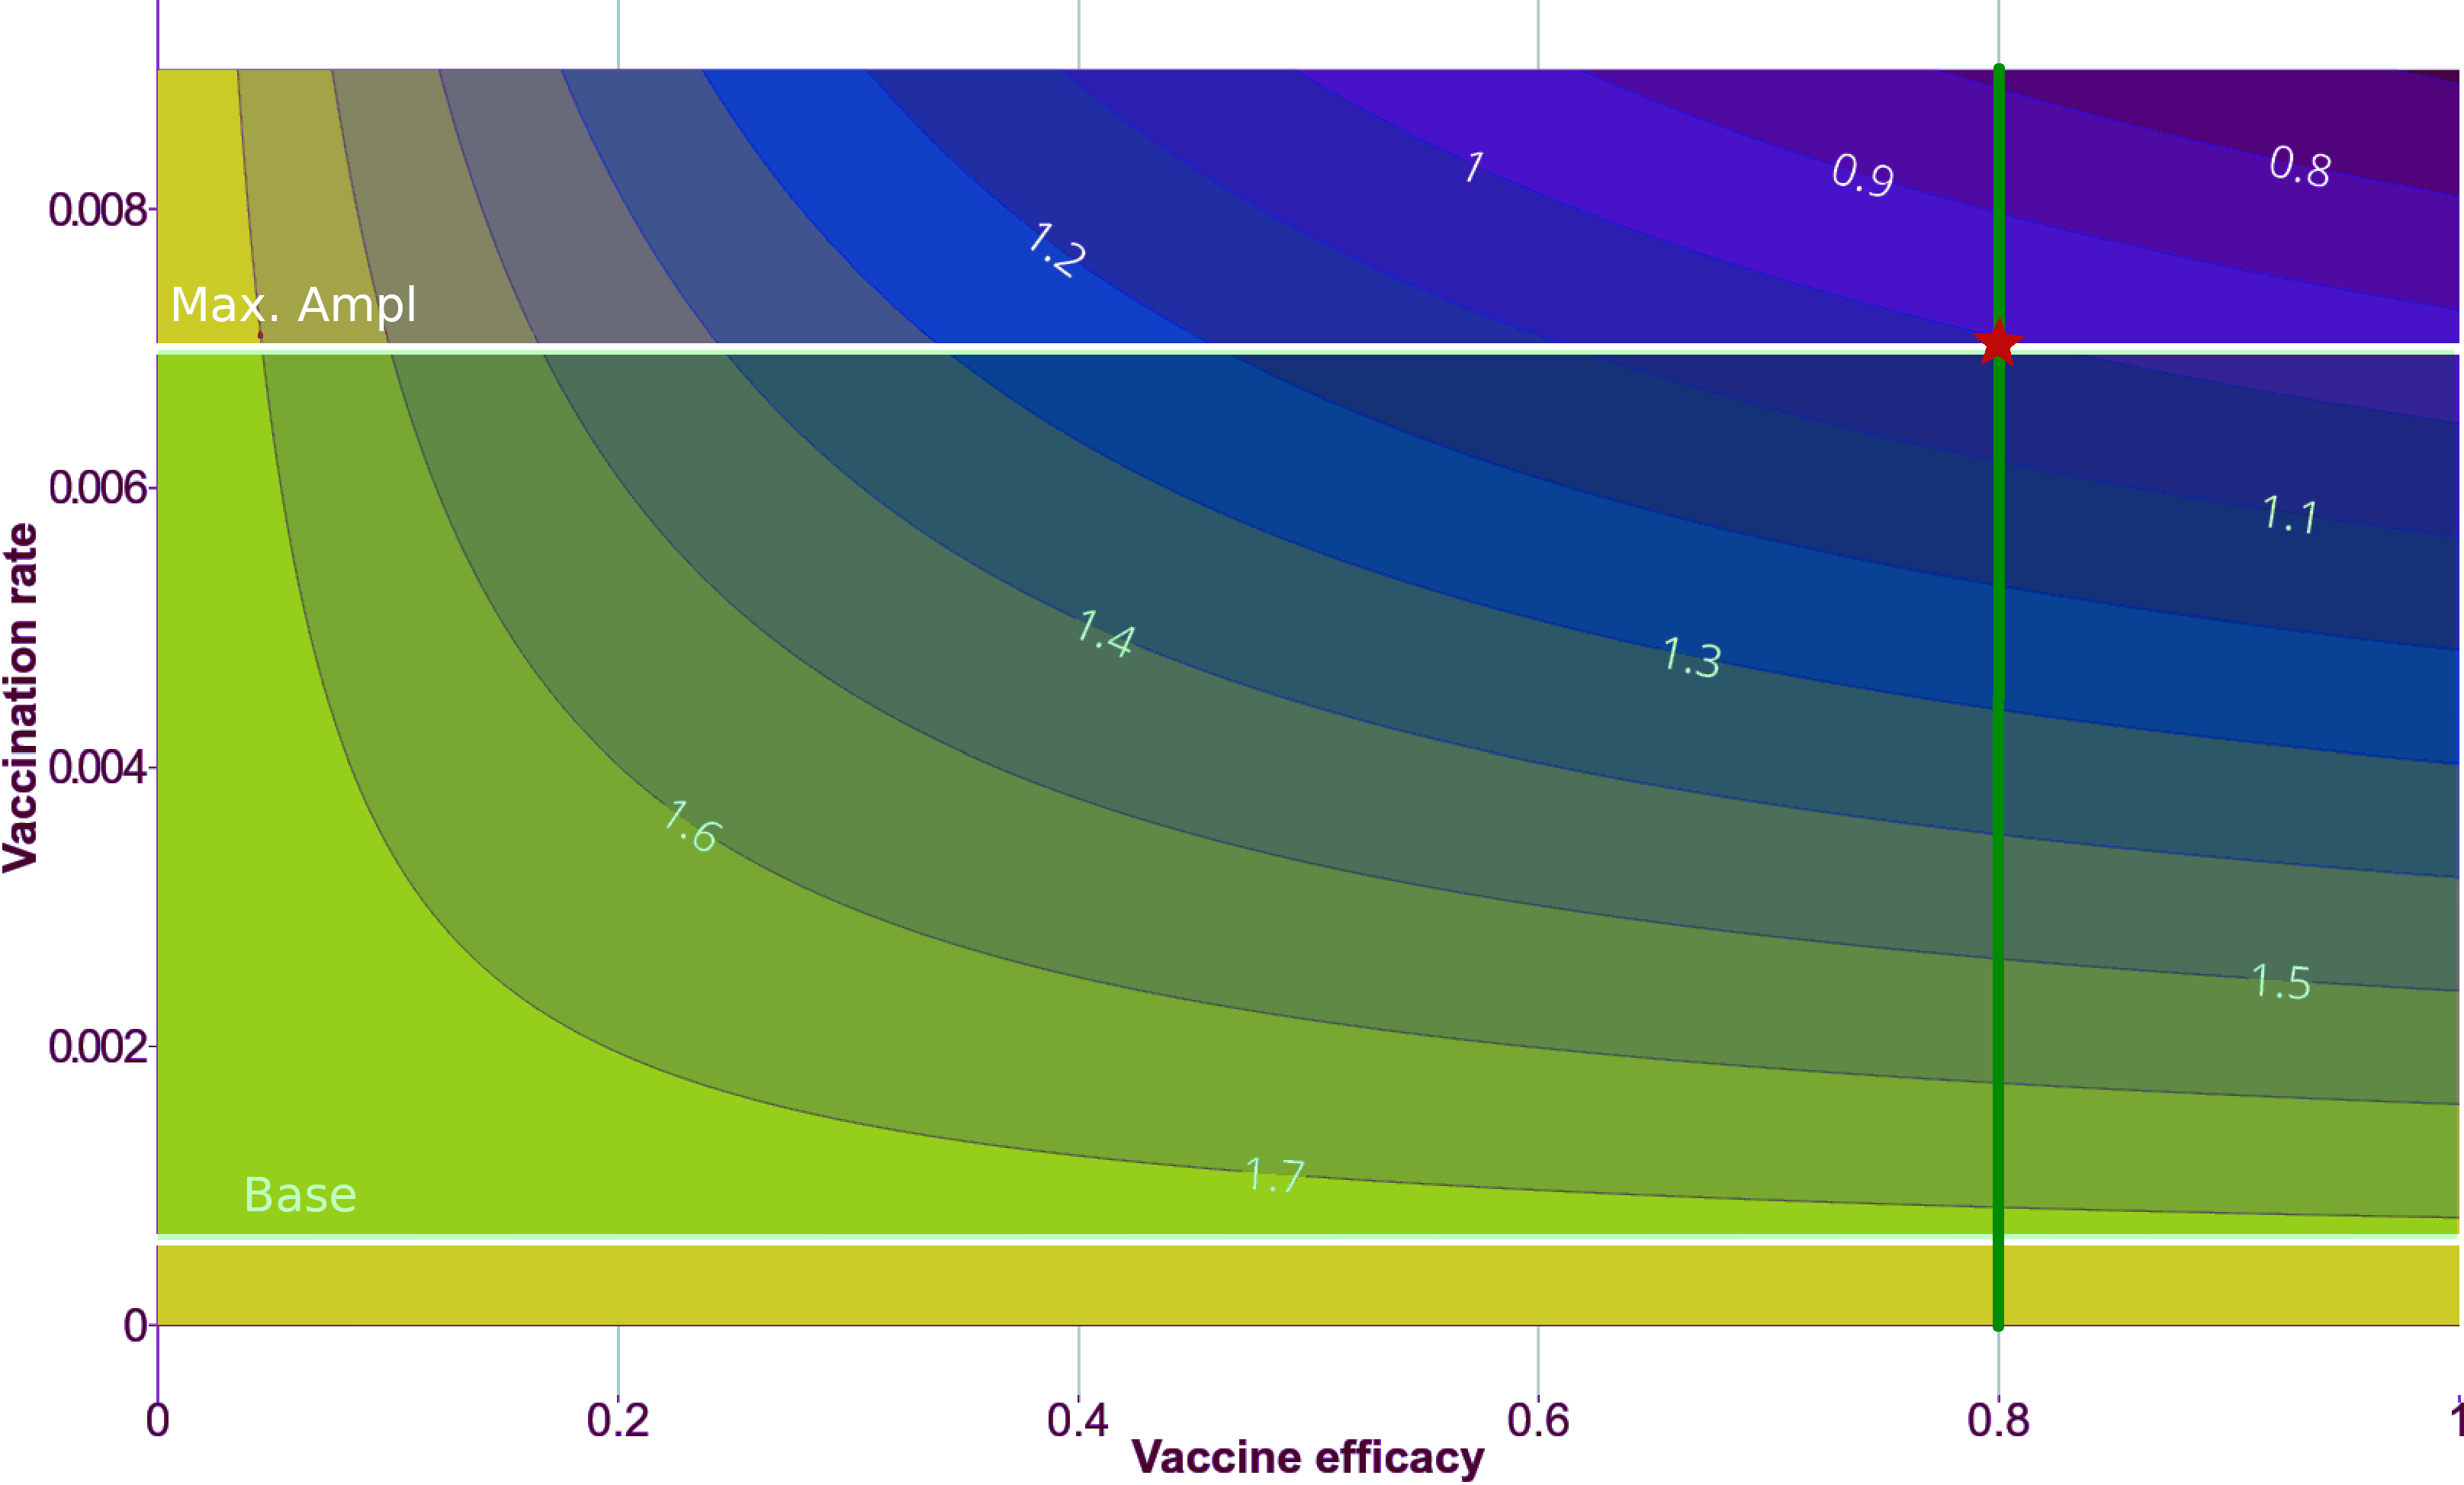
\includegraphics[scale=.65,%
%              keepaspectratio]{assets/RvAnimation/r_zero_vac_level_plots05.png}
%         }
%     \end{textblock*}
% %
%     \begin{textblock*}{40mm}(3mm, 65mm)
%         \only<8->{
%             \begin{graybox}{$\lambda_V$ estimation}
%                 Given a fixed coverage $X_{cov}$ and
%                 time horizon $T$
%                 $$
%                     1 - \exp(- \lambda_V T) = X_{cov}
%                 $$
%             \end{graybox}
%         }
%     \end{textblock*}
%     \begin{textblock*}{37mm}(90mm, 10mm)
%         \only<9->{
%             \begin{greenbox}{
%                 $X_{COV}: \SI{20}{\percent} \\
%                 T:\SI{1}{year}$
%         }
%         $
%             \lambda_V \approx 0.000611352
%         $
%         \tcblower
%         \only<10->{
%             \hspace*{-.5cm}
%             To decrease  {$R_V\leq 1$},
%             \\
%             \hspace*{-.5cm}
%             we require
%             $$
%                 \epsilon \geq 0.8, 
%                 \quad 
%                 \lambda_V 
%                 \geq \num{0.007}
%             $$
%         }
%            \end{greenbox}
%         }
%     \end{textblock*}
\end{frame}
    \section{Optimal Control Problem (OCP)}
        %!TEX root = ../main.tex
\begin{frame}{The Optimal Control Problem}
    \setlength{\leftmargini}{1mm}
    \begin{textblock*}{130mm}(0mm, 20mm)
        \only<1>{

            \includegraphics[scale=0.125,%
                keepaspectratio]{assets/%
                SchemeModel_withoutVaccination01.png}
        }
        \only<2>{
            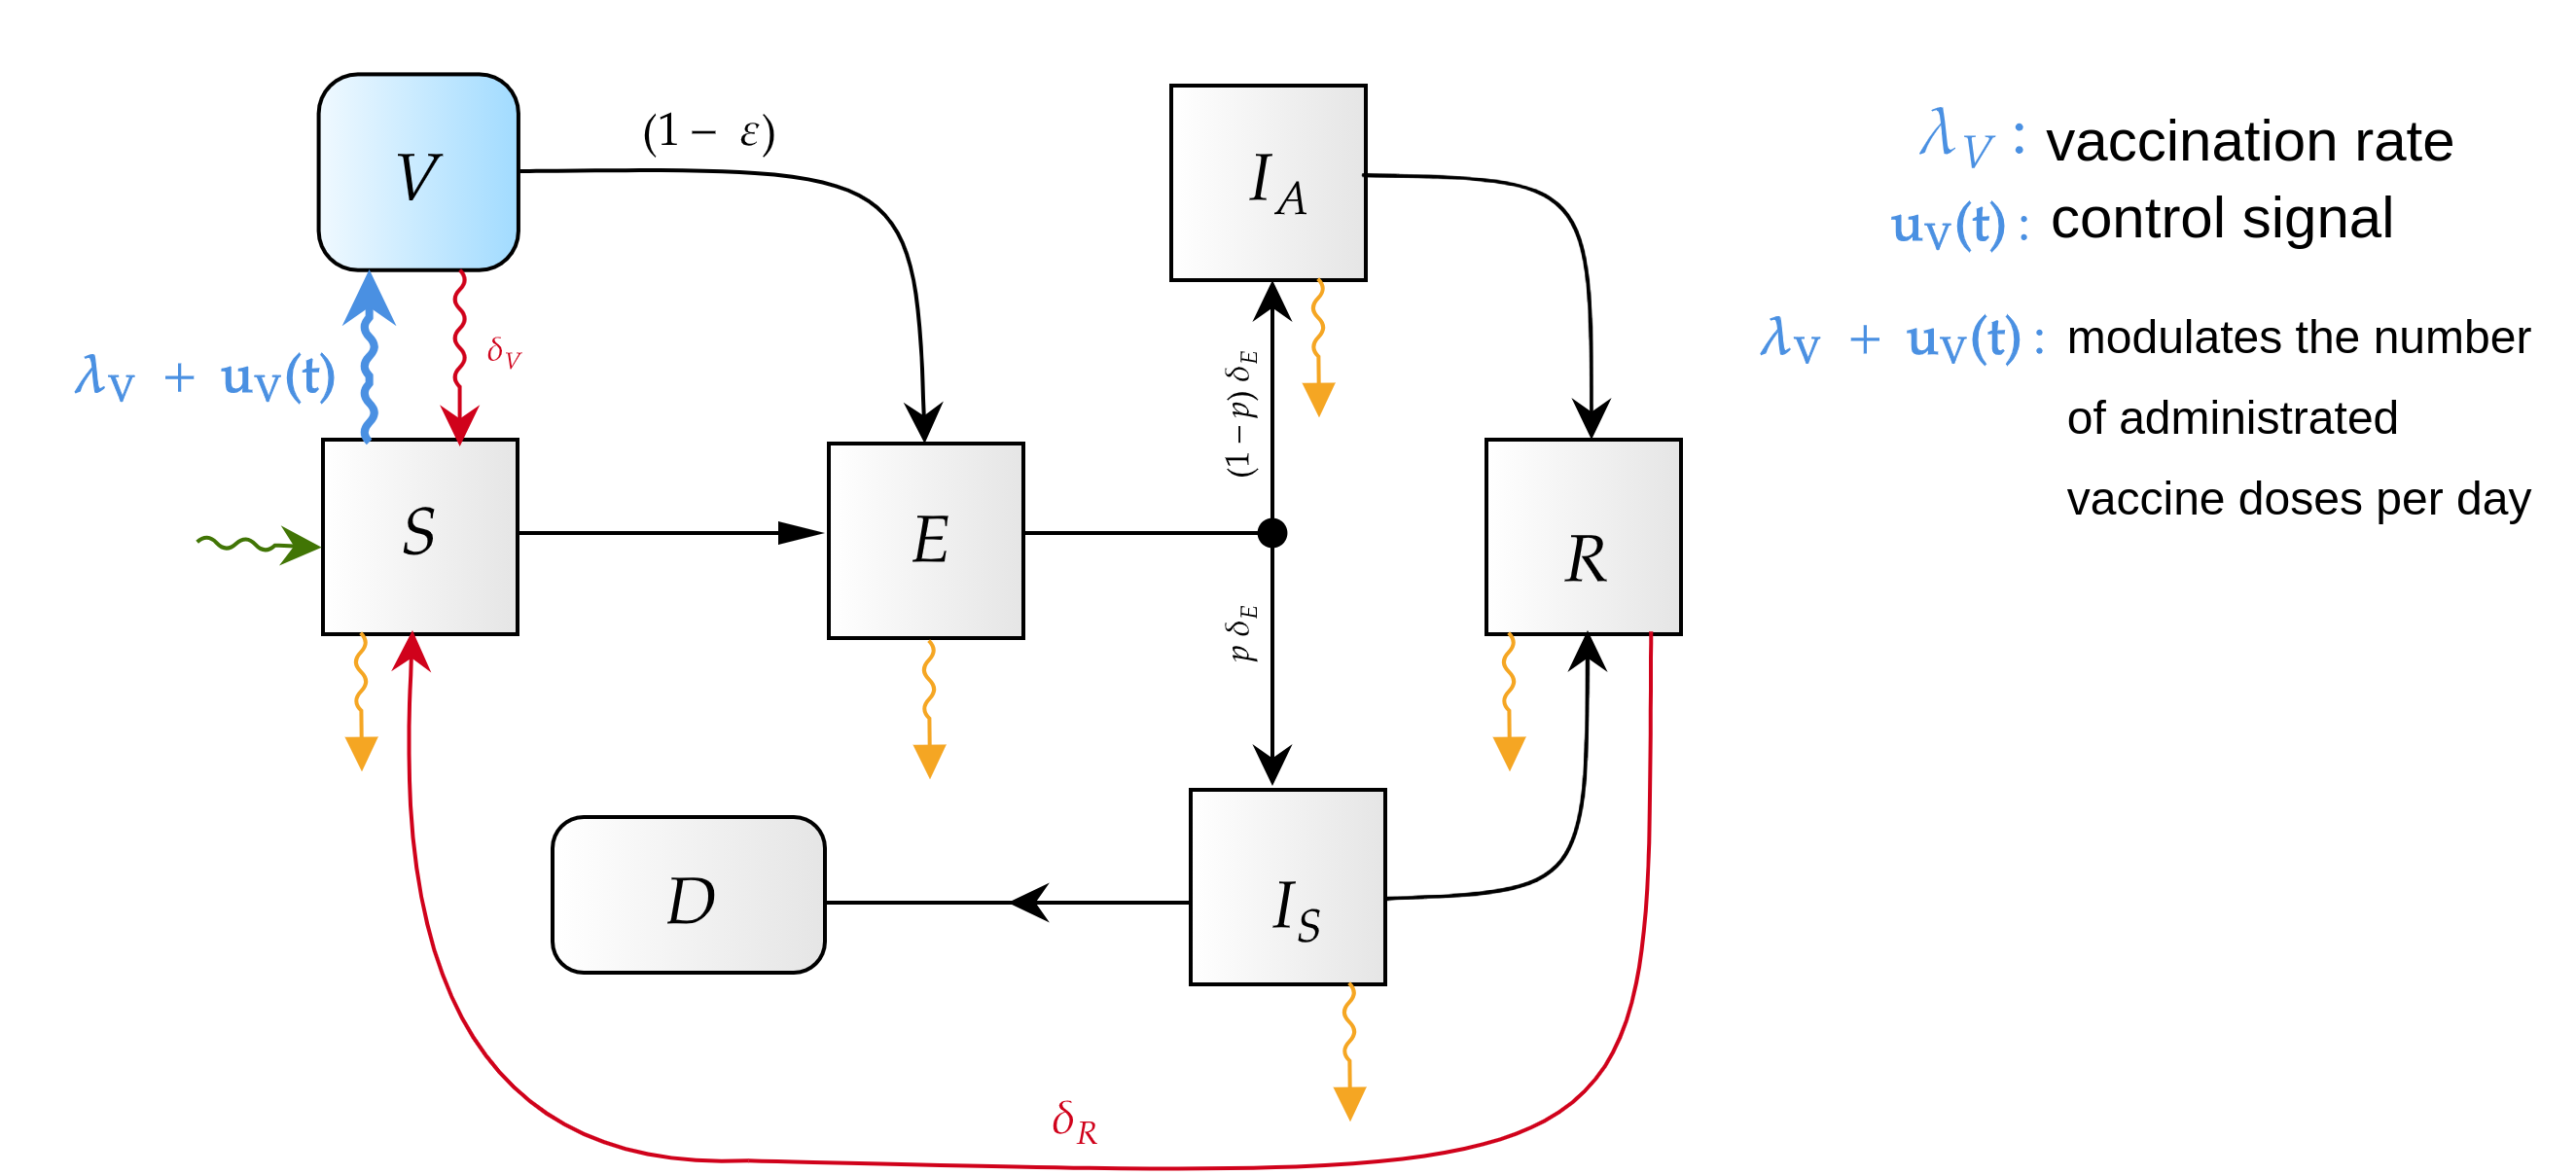
\includegraphics[scale=.125,%
                keepaspectratio]{assets/SchemeModel01.png}
        }
        \only<3>{
            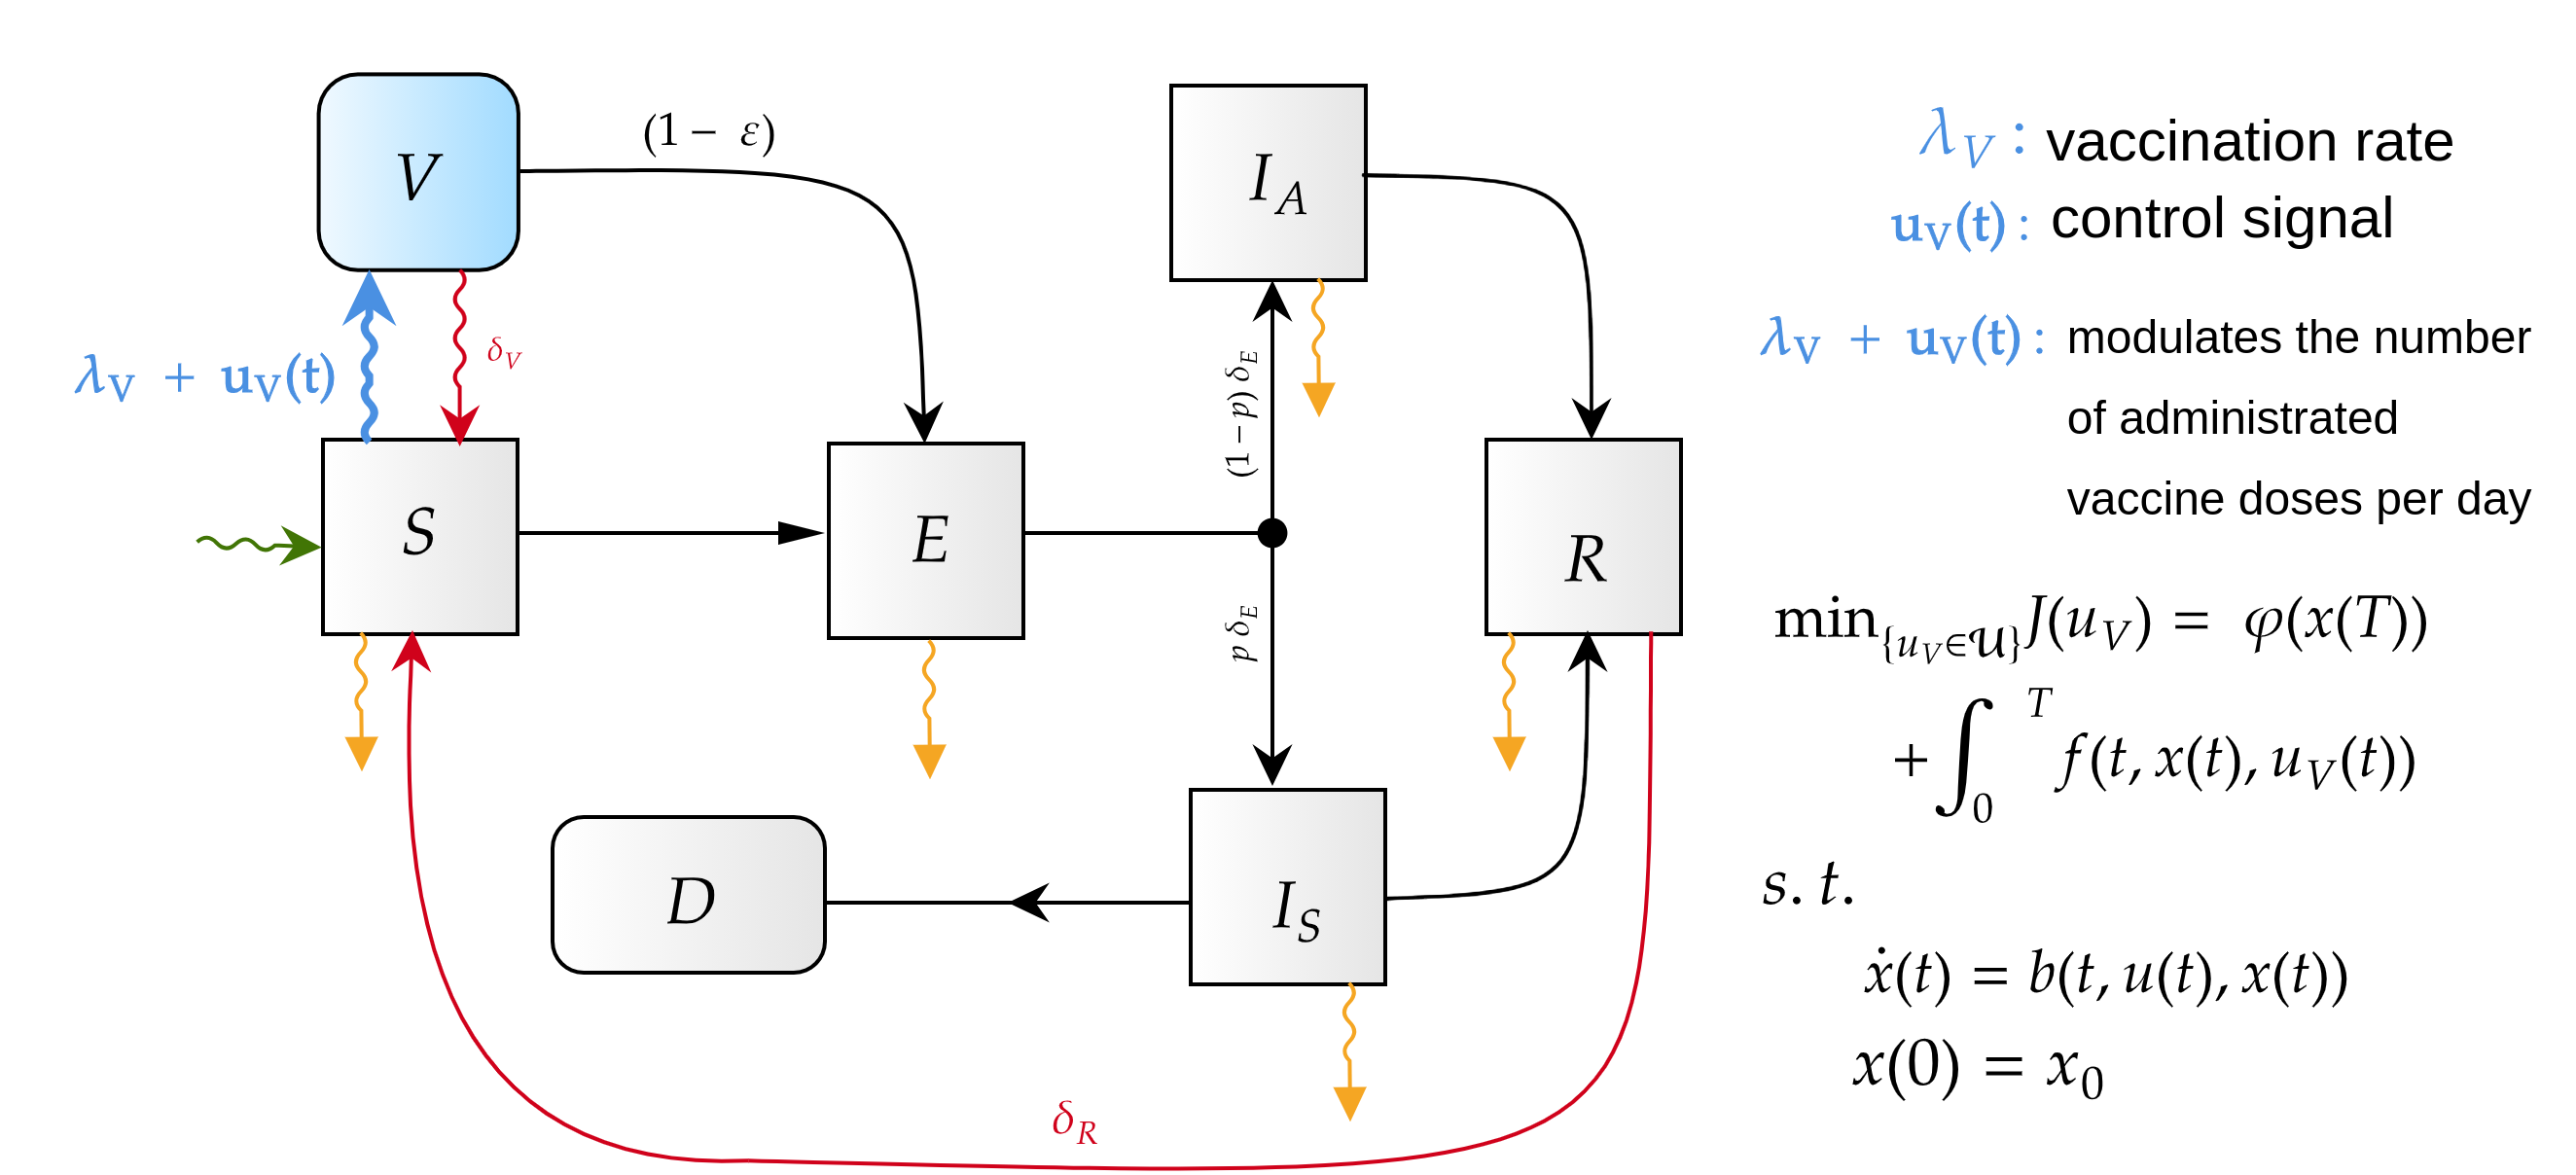
\includegraphics[scale=.125,%
                keepaspectratio]{assets/SchemeModel02.png}
        }
    \end{textblock*}
\end{frame}
\begin{frame}{The disability-adjusted life year (DALY)}
    \begin{textblock*}{120mm}(5mm,10mm)
        %
        \begin{graybox}{{$DALY(c,s,a,t) = YLL(c,s,a,t) + YLD(c,s,a,t)$}}
            For given cause c, age a, sex s and year t
            \begin{description}
                \item[$YLL:$] Years of life lost due to premature death.
                    $$
                        YLL(c,s,a,t) = N(c,s,a,t) \times L(s,a)
                    $$
                    \begin{itemize}
                         \item
                             $N(c,s,a,t):$ is the number of 
                             deaths due to the cause $c$ 
                         \item
                             $L(s,a):$ is a standard loss 
                             function specifying years of life lost 
                    \end{itemize}
                 \item[$YLD:$] Years of life list due to disability   
                     $$
                         YLD(c,s,a,t) = I(c,s,a,t) \times DW(c,s,a) 
                         \times L(c,s,a,t)
                     $$
                    \begin{itemize}
                        \item
                            $I(c,s,a,t):$ number of incident cases for cause c
                        \item
                            $DW(c,s,a):$ disability weight for cause c
                        \item
                            $L(c,s,a,t):$  average duration of the case 
                            until remission or death (years)
                    \end{itemize}
            \end{description}
       \end{graybox}
       \begin{equation*}
            \begin{aligned}
             & \only<2->{\min_{u_V  \in \mathcal{U}[0, T]}}
             J(u_V) :=
             \only<3->{
                \underbrace{a_D ( D(T) - D(0))}_{:=YLL}  +
                \underbrace{a_S (Y_{I_S}(T) - Y_{I_S}(0))}_{:=YLD}
             }
            \end{aligned}
       \end{equation*}        
    \end{textblock*}
    \end{frame}
    %
    %
    \begin{frame}{Optimal Control Problem}
    \begin{textblock*}{120mm}(10mm,10mm)
        \only<1-3>{
            \begin{equation*}
                    \begin{aligned}
                             &
                             \textcolor<1>{orange}{%
                                \min_{u_V  \in \mathcal{U}[0, T]}
                                J(u_V) :=
                                    \underbrace{a_D ( D(T) - D(0))}_{:=YLL}  +
                                    \underbrace{
                                        a_S (Y_{I_S}(T) - Y_{I_S}(0))
                                    }_{:=YLD}
                            }
                        \\
                             & 
                             \textcolor<2>{orange}{
                                u_V(\cdot)   \in [u_{\min}, u^{\max}],
                            }
                        \\
                            &
                            \textcolor<3>{orange}{
                                \kappa I_S(t)  
                                \leq B, \quad \forall t \in [0, T],
                             }
                        %}
                    \end{aligned}
            \end{equation*}
        }
    \end{textblock*}    
    \begin{textblock*}{85mm}(0mm,10mm)        
        \only<4->{
            \begin{equation*}
                \begin{aligned}
                    &\min_{u_V  \in \mathcal{U}[0, T]}
                    J(u_V) :=
                    %\int_0 ^ T
                    % a_D D(s) + a_S Y_{I_S}(s) ds
                    a_D ( D(T) - D(0)) +
                    a_S (Y_{I_S}(T) - Y_{I_S}(0))
                    \\
                    \text{s.t.} &
                    \\
                    &f_{\lambda}
                    :=
                    \frac{\beta_S I_S + \beta_AI_A}{\bar{N}}
                    \\
                    S'(t)
                    &=
                    \mu \bar{N} + \delta_V V + \delta_R R
                    \\
                    &-
                    (f_{\lambda} + \mu + \lambda_V +  u_V(t)) S
                    \\
                    E'(t)
                    &=
                    f_{\lambda} (S + (1-\epsilon) V)
                    - (\mu+\delta_E) E
                    \\
                    I'_S(t)
                    &=p
                    \delta_E
                    E-(\mu + \alpha_S) I_S
                    \\
                    I'_A(t)
                    &= (1 - p) \delta_E E-(\mu + \alpha_A) I_A
                    \\
                    R'(t)
                    &= (1 - \theta) \alpha_S I_S + \alpha_A I_A
                    - (\mu + \delta_R) R
                    \\
                    D'(t)&=
                    \theta \alpha_S I_S
                    \\
                    V'(t)&=
                    (\lambda_V + u_V(t)) S -
                    \left(
                    (1 -\epsilon) f_{\lambda} V +
                    \mu + \delta_V
                    \right) V
                    \\
                    X'(t)&=
                    (\lambda_V + u_V(t))(S + E + I_A + R)           
                \end{aligned}
            \end{equation*}
        }
    \end{textblock*}
%
    \begin{textblock*}{60mm}(70mm, 30mm)
        \only<4->{
            \begin{equation*}
                \begin{aligned}
                    S(0) &= S_0, \ E(0) = E_0, \ I_S(0) = I_{S_{0}},
                    \\
                    I_A(0) &= I_{A_{0}}, \ R(0) = R_0, \ D(0) = D_0,
                    \\
                    V(0) &= 0, \ X(0) = 0, \ X(T) = x_{coverage},
                    \\
                    u_V(\cdot) & \in [u_{\min}, u^{\max}],
                    \\
                    \kappa I_S(t) & \leq B, \quad \forall t \in [0, T],
                    \\
                    \bar{N}(t) &= S + E + I_S + I_A + R + V.
                \end{aligned}
            \end{equation*}
        }
    \end{textblock*}
\end{frame}
    \section{Numerical Results}
        %!TEX root = ../main.tex
\begin{frame}{Vaccine efficacy} 
\begin{table}[htb]
            \centering
            \begin{tabular}{%
                p{3.2cm} 
                p{2cm} 
                p{3.1cm} 
                P{1.5cm}
            }
            \toprule
            \textbf{Developer} &
            \textbf{Vaccine Name} &
            \textbf{Efficacy \%, (95\% CI)} &  
            %\textbf{Status} & 
            \textbf{Reference}
                \\
                 \midrule
                \\
                    Pfizer-BioNTech
                        & BNT162b2 
                        & \num{95} (\num{90.3}–\num{97.6})
                        %& Approved for emergency use in the USA, Mexico, 
                        % Germany, UK, and other countries
                        & \cite{Dagan2021} %\cite{vaccine_tracker2020}
                \\
                    Gamaleya Institute
                        & Sputnik V 
                        & \num{91.6} (\num{85.6}–\num{95.2}) 
                        %& Early use in Russia. Emergency use Mexico an other 
                        %countries.
                        & \cite{Logunov2021}
                \\
                    Oxford University-AztraZeneca
                        & AZD1222
                        & \num{74.6} (\num{41.6}-\num{88.9}) 
                        %& Approved for emergency use in the USA, Mexico, 
                        & \cite{Emary2021}
                \\
                    Johnson \& Johnson$^{*}$
                        & Ad26.COV2.S
                        & \SI{57}{\percent}, \SI{66}{\percent} or \SI{72}{\percent}
                        %& Approved for emergency use in the USA, Mexico, 
                        & \cite{johnsonandjohnson}
                \\
                    Sinovac Biotech$^{*}$
                        & CoronaVac
                        & \SI{50.4}{\percent}
                       % & Approved in China. Emergency use in Brazil, other 
                       % countries.
                        &\cite{vaccine_tracker2020}
                \\
            \bottomrule
            \end{tabular}
            \caption{Vaccine efficacy of some 
            of the approved developments for emergency use. $(^{*})$ No available information about the confidence intervals.}
            \label{tbl:vaccine-efficacy-portfolio}
        \end{table}
\end{frame}

% \begin{frame}{Simulation Results}
%     %TODO: Calculate vaccine dosis price according to CDMX report
%     \begin{center}
%         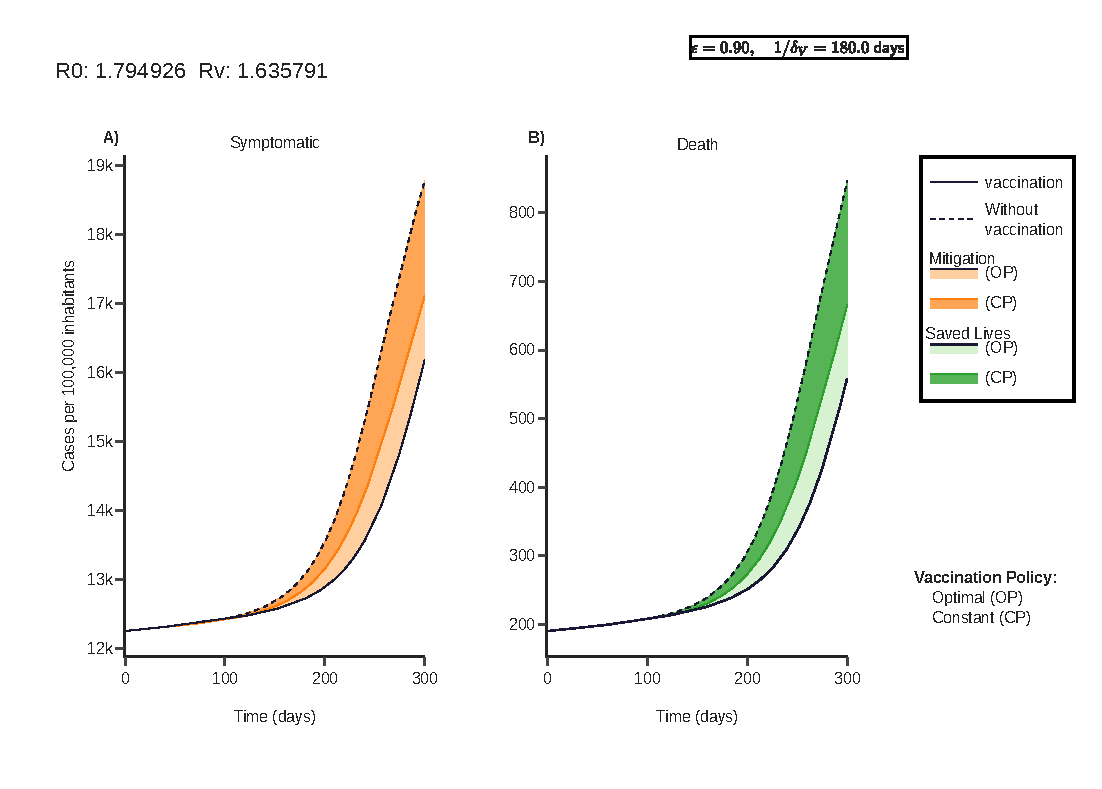
\includegraphics[scale=.65, keepaspectratio]{assets/incidence_fig}
%     \end{center}
% \end{frame}

% \begin{frame}{Simulation Results}
%     \begin{textblock*}{130mm}(-1mm, 5mm)
%         \only<1>{
%             \begin{center}
%                 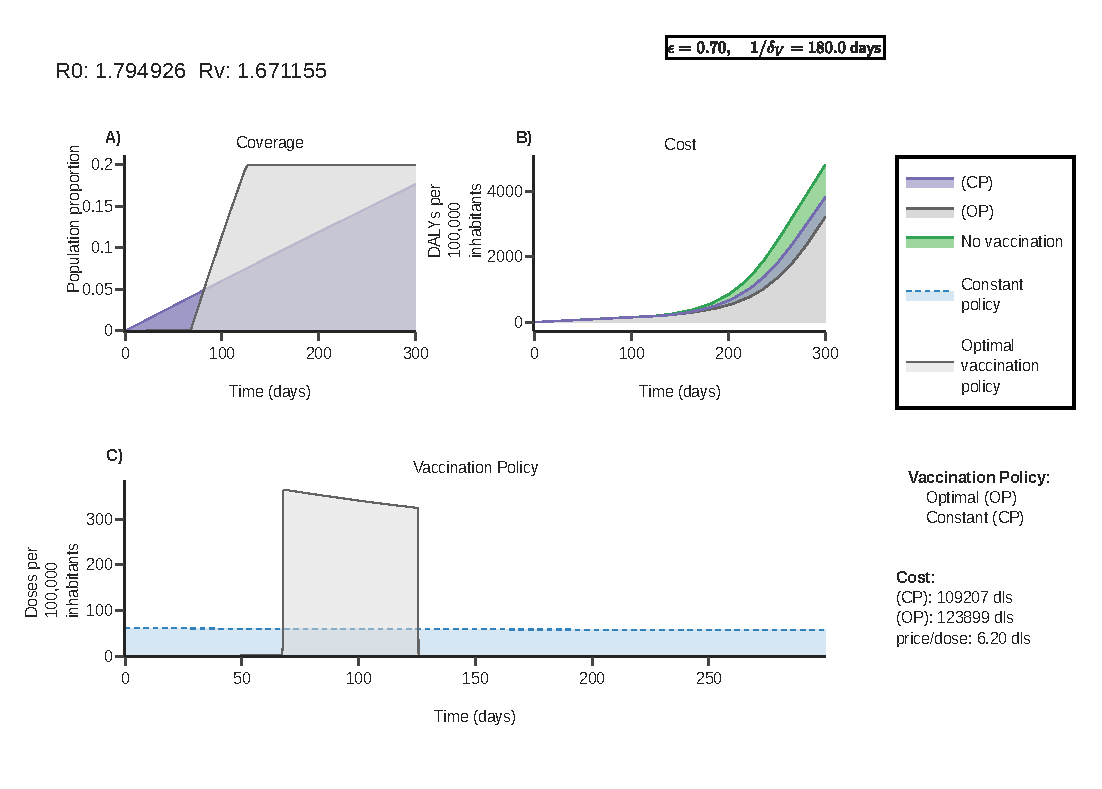
\includegraphics[scale=.62,
%                 keepaspectratio]{assets/optimal_signal_fig01.pdf}
%             \end{center}
%         }
%         \only<2>{
%             \begin{center}
%                 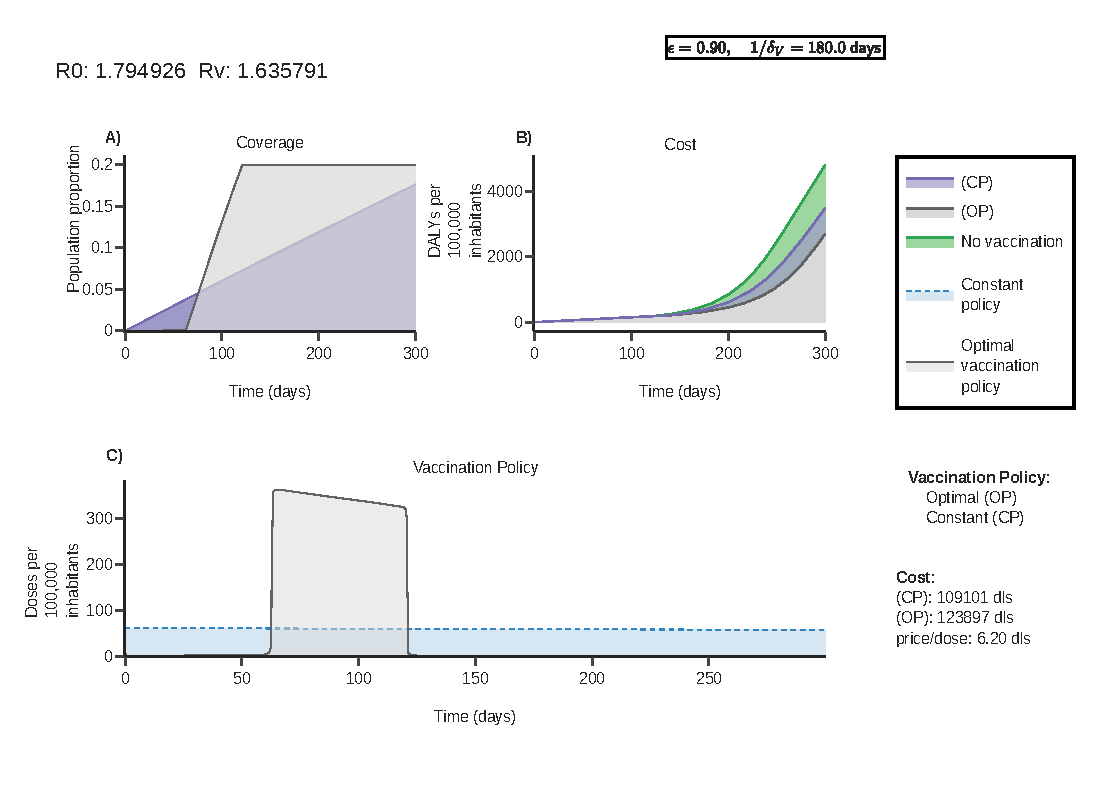
\includegraphics[scale=.62,
%                 keepaspectratio]{assets/optimal_signal_fig02.pdf}
%             \end{center}
%         }
%     \end{textblock*}
% \end{frame}
%%%%%%%%%%%%%%%%%%%%%%%%%%%%%%%%%%%%%%%%%%%%%%%%%%%%%%%%%%%%%%%%%%%%%%%%%%%%%%%%

        %!TEX root = ../main.tex
\begin{frame}{The response of COVID-19 burden due to vaccine efficacy}
    \begin{textblock*}{127mm}(0mm, 10mm) 
        \begin{block}{%
            $
                (x_{coverage},
                T, \varepsilon,\delta_{V}^{-1}, \delta_{R}^{-1}):
            $%
            \qquad
            [
                \SI{50}{\percent},
                \SI{365}{days},
                $\star$,
                \SI{730}{days},
                \SI{365}{days}
            ]
        }
        \only<1>{

            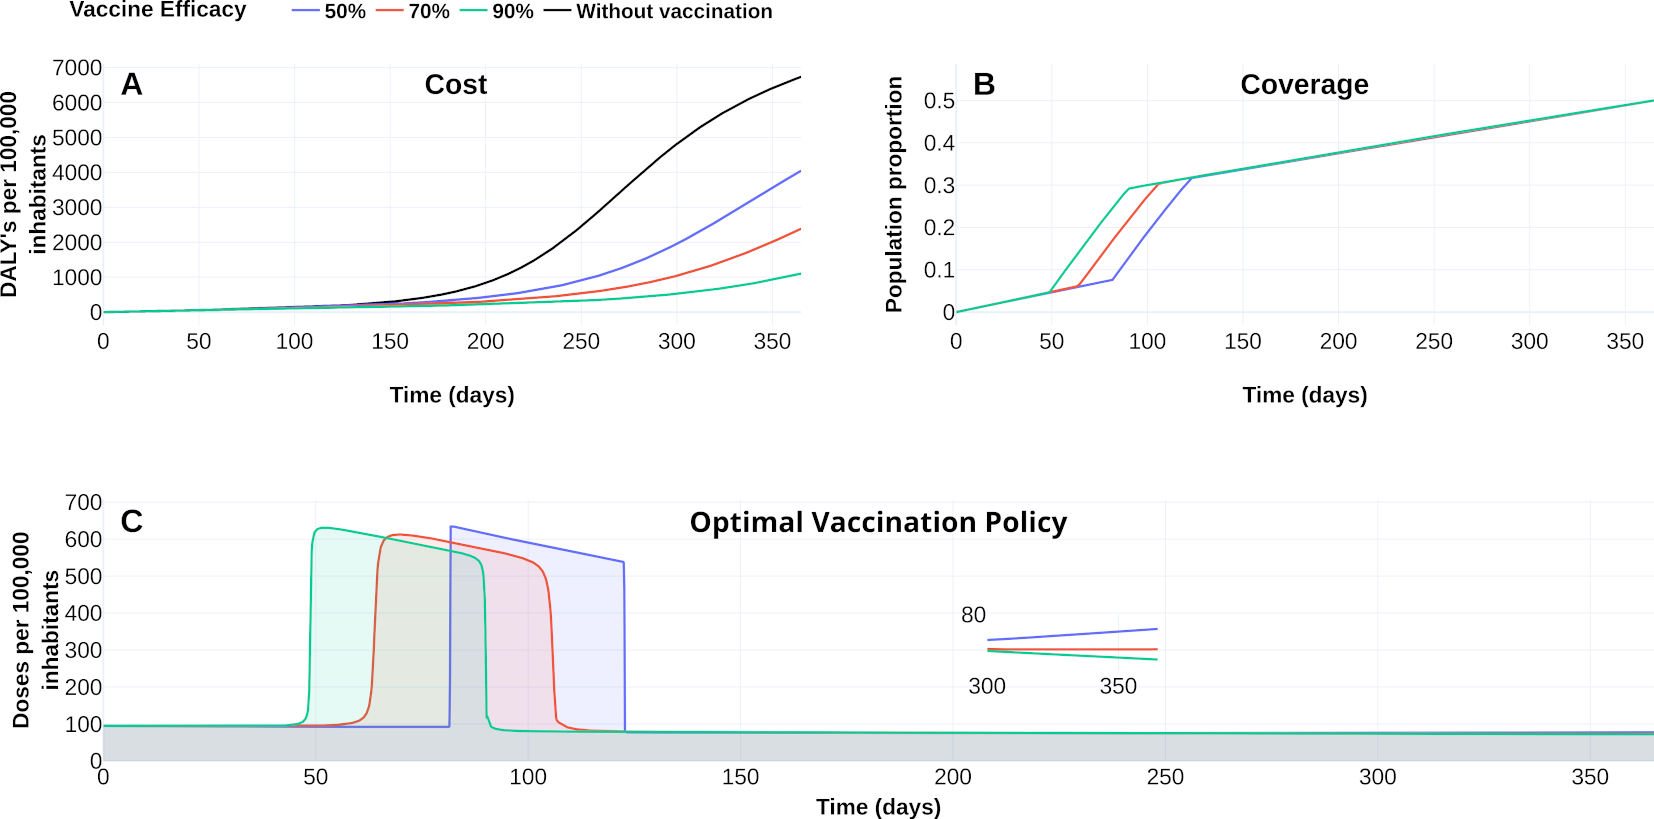
\includegraphics[width=\textwidth,keepaspectratio]{%
            assets/efficacy01.png}
        }
        \only<2>{
            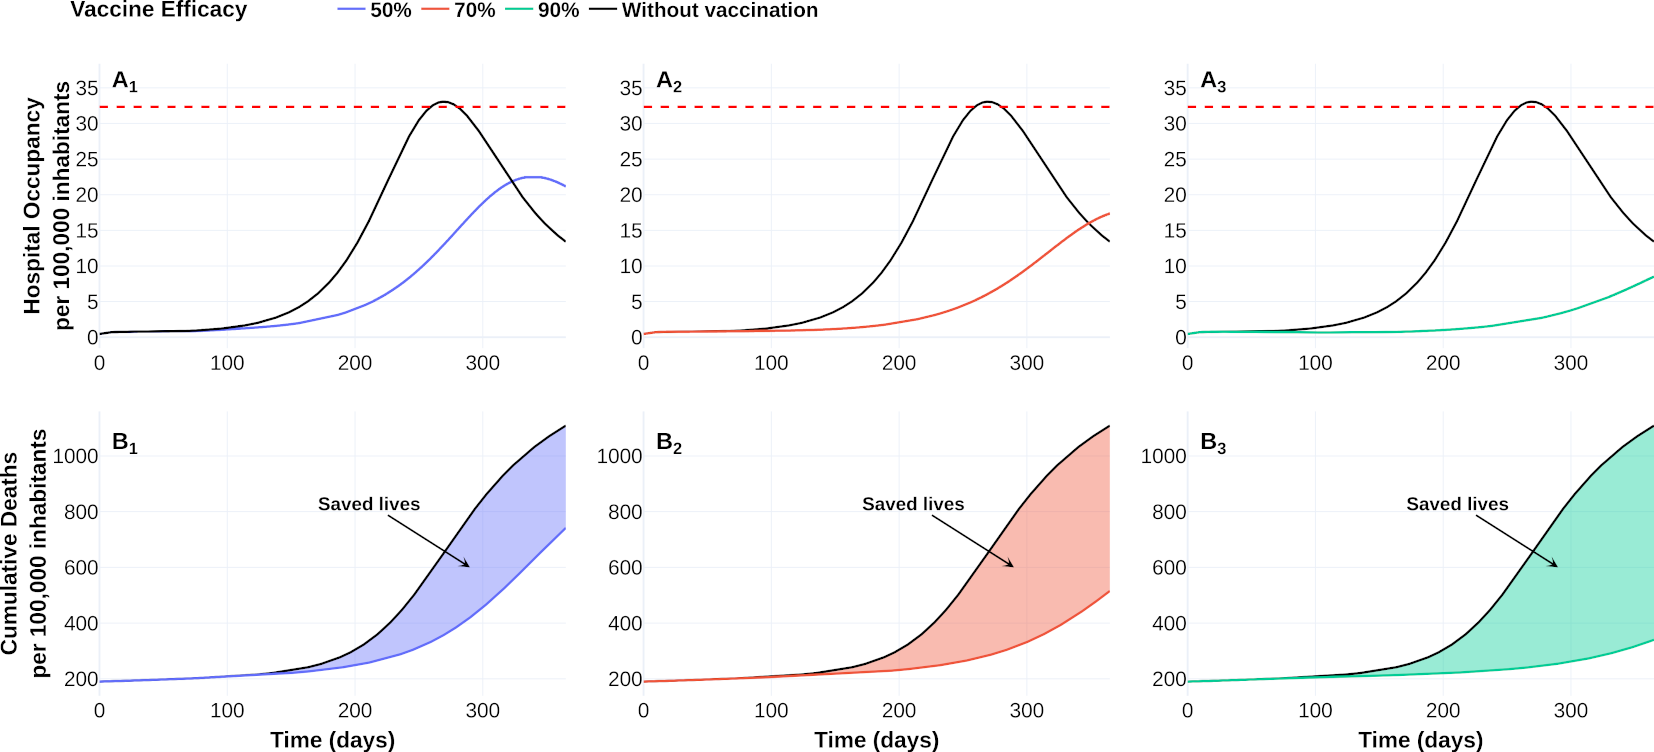
\includegraphics[width=\textwidth,keepaspectratio]{%
            assets/efficacy02.png}
        }
        \end{block}
    \end{textblock*}
\end{frame}
        %!TEX root = ../main.tex
\begin{frame}{The response of COVID-19 burden due to vaccine-immunity}
    \begin{textblock*}{127mm}(0mm, 10mm) 
        \begin{block}{%
            $
                (x_{coverage},
                T, \varepsilon,\delta_{V}^{-1}, \delta_{R}^{-1}):
            $%
            \qquad
            [
                \SI{50}{\percent},
                \SI{365}{days},
                \SI{90}{\percent},
                $\star$,
                \SI{365}{days},
            ]
        }
        \only<1>{

            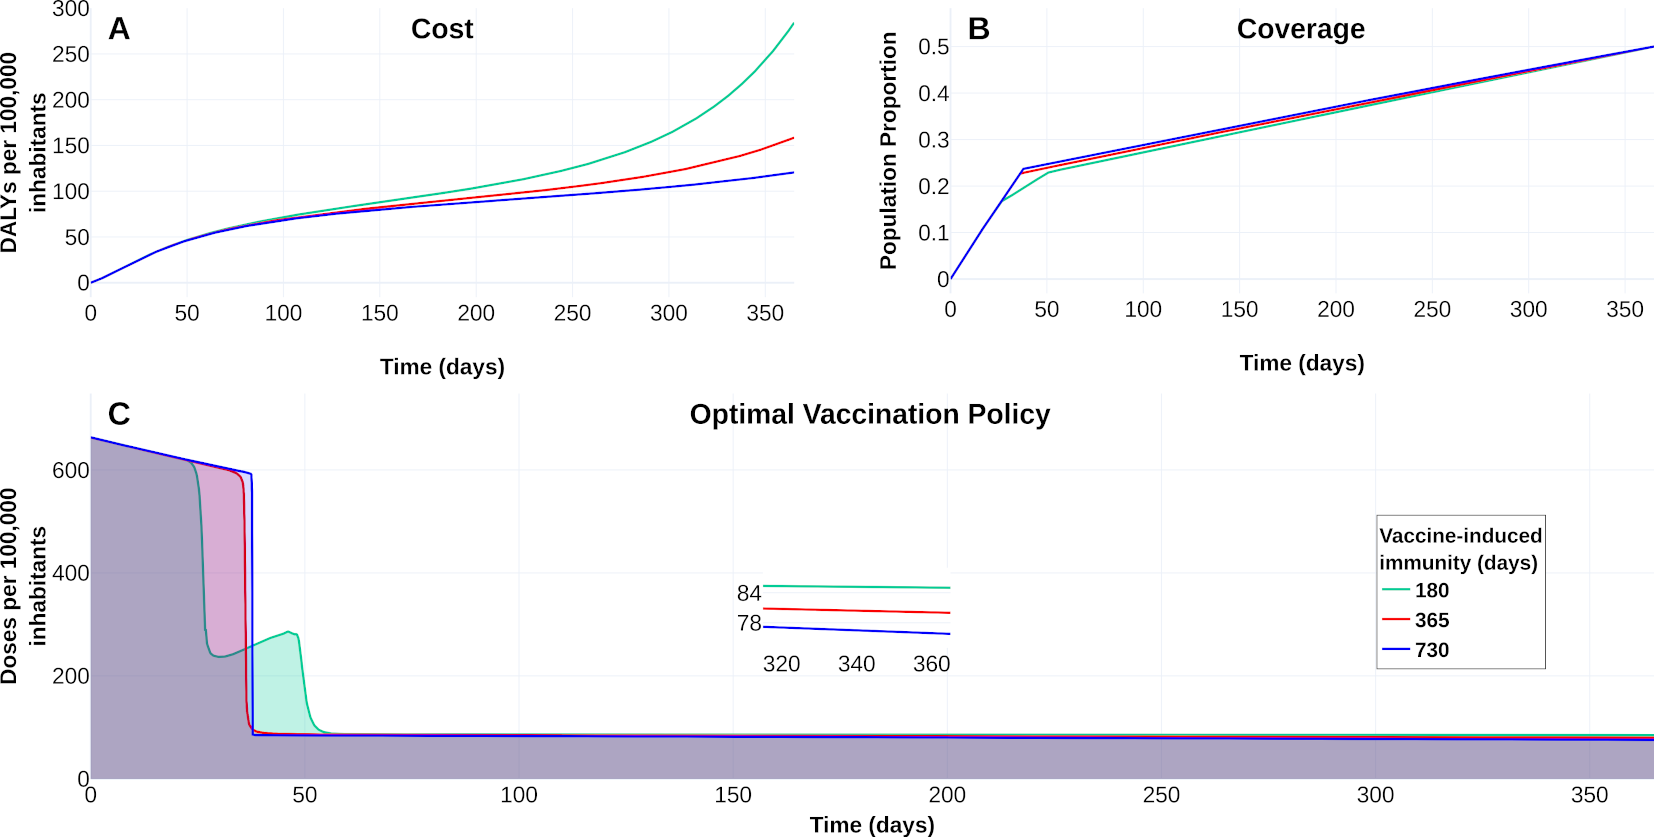
\includegraphics[width=\textwidth,keepaspectratio]{%
            assets/vaccine-immunity01.png}
        }
        \only<2>{
            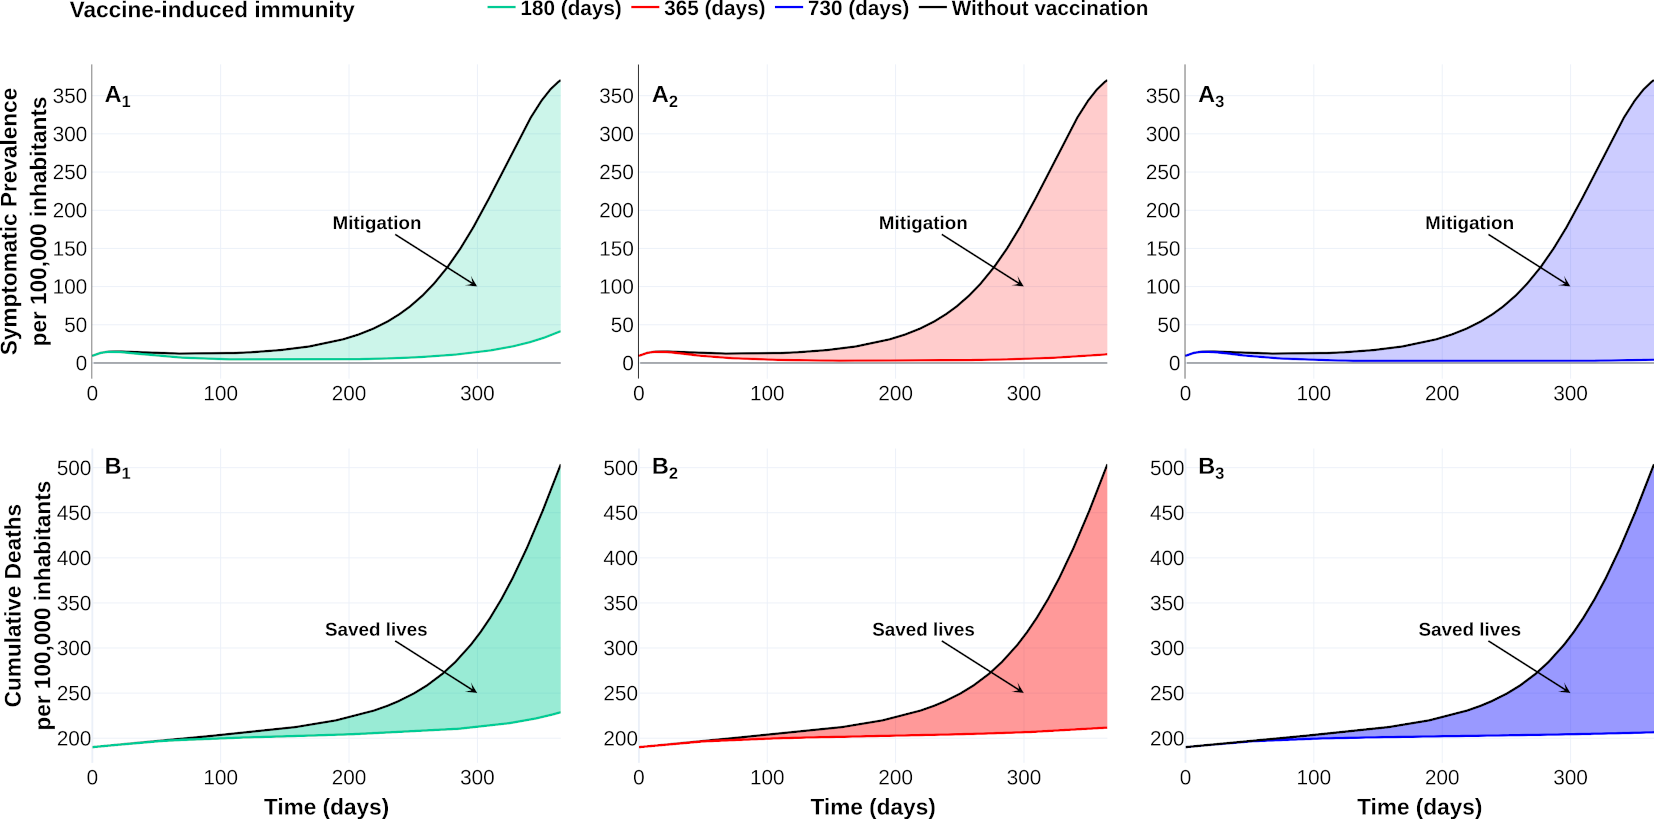
\includegraphics[width=\textwidth,keepaspectratio]{%
            assets/vaccine-immunity02.png}
        }
        \end{block}
    \end{textblock*}
\end{frame}
        %!TEX root = ../main.tex
\begin{frame}{The response of COVID-19 burden due to natural-immunity}
    \begin{textblock*}{127mm}(0mm, 10mm) 
        \begin{block}{%
            $
                (x_{coverage},
                T, \varepsilon,\delta_{V}^{-1}, \delta_{R}^{-1}):
            $%
            \qquad
            [
                \SI{50}{\percent},
                \SI{365}{days},
                \SI{90}{\percent},
                \SI{730}{days},
                $\star$%
            ]
        }
        \only<1>{

            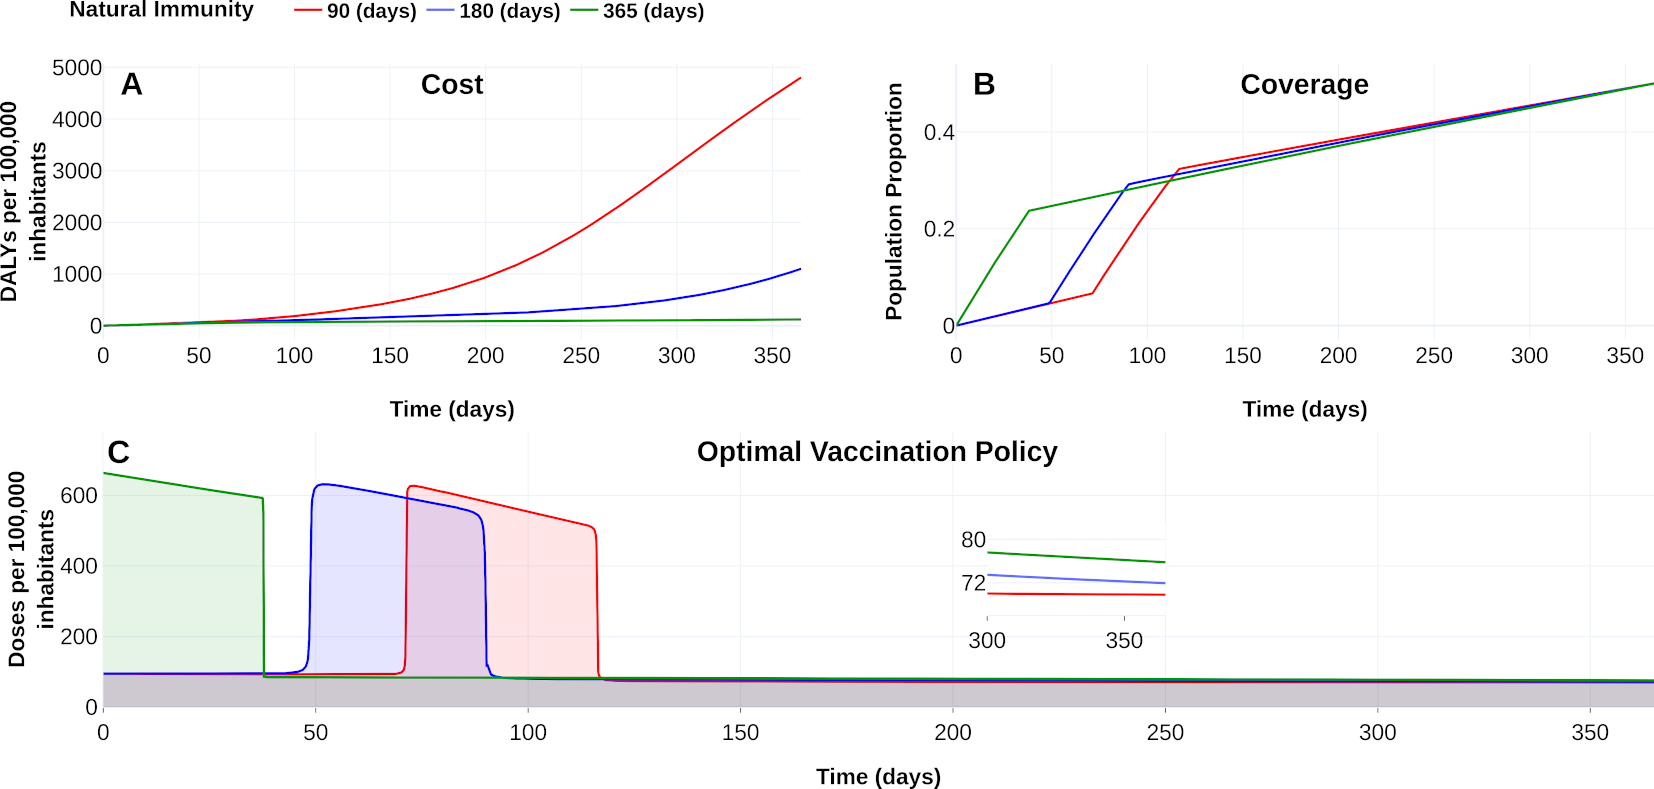
\includegraphics[width=\textwidth,keepaspectratio]{%
            assets/natural-immunity01.png}
        }
        \only<2>{
            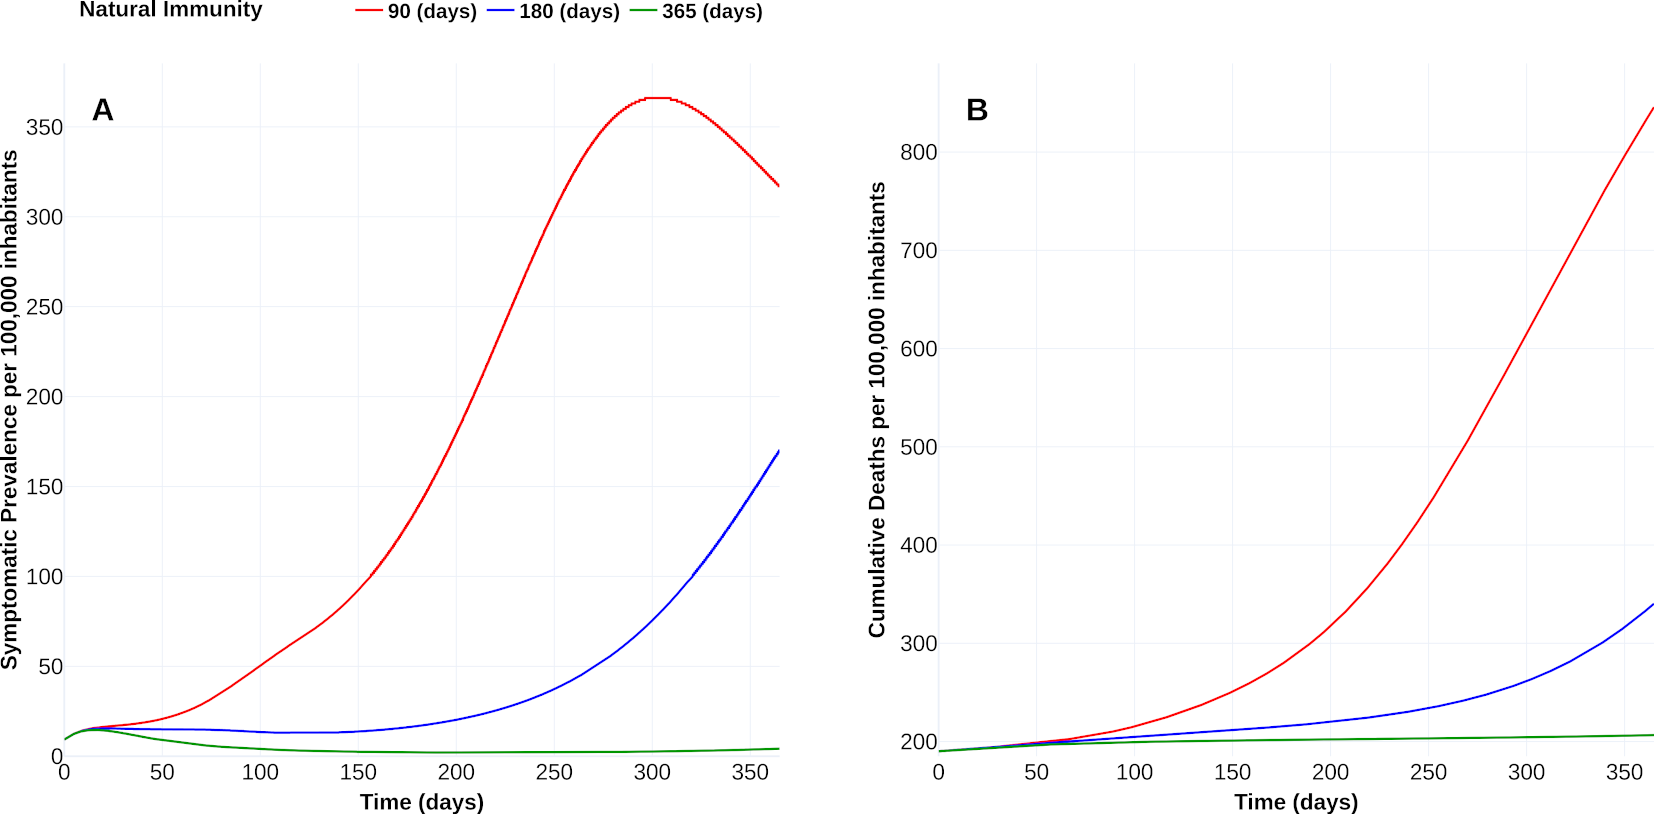
\includegraphics[width=\textwidth,keepaspectratio]{%
            assets/natural-immunity02.png}
        }
        \end{block}
    \end{textblock*}
\end{frame}
    \section{Final comments}
        %!TEX root = ./main.tex
\begin{frame}{Important questions}
    \begin{textblock*}{90mm}(20mm, 20mm)  
        \begin{itemize}
            \item[($\star$)]<+->
                Optimal vaccination strategies in terms of target groups 
                and under different possible supply scenarios 
                \begin{itemize}
                    \item[$\bullet$]
                        Two or more vaccine platforms
                    \item[$\bullet$]
                        Multi-doses
                \end{itemize}
            \item[($\star$)]<+->
                Potential reduction in infectiousness of 
                breakthrough infections among vaccinated
                individuals
            \item[($\star$)]<+->
                Potential differences in vaccine efficacy against 
                mild or severe/fatal COVID-19 disease
        \end{itemize}
    \end{textblock*}
\end{frame}

\begin{frame}{Team CONACYT, UNISON, ITSON, UNAM }
    \begin{center}
        \begin{tabular}{rl}
            %\toprule
            Working group
            \\
            \midrule
            Dr. Saúl Díaz Infante Velasco
            &
                CONACYT-UNISON
            \\
            Dr. Manuel A. Acu\~na Zegarra
            &
                UNISON
            \\
            Dr. Daniel Olmos Liceaga
            &
                UNISON
            \\
            Dr. David Baca Carrasco
            &
                ITSON
           \\
           Dr. David Gonz\'alez-S\'anchez
            &
            CONACYT-UNISON
           \\
           Dr. Francisco Pe\~nu\~nuri
           & UADY
           \\
            M.C. Gabriel Salcedo-Varela
            & UNISON
            \\
            \\
           Adviser
           \\
           \midrule
            Dr. Jorge X. Velasco Hern\'andez
            &
            UNAM-Juriquilla
            
        \end{tabular}
    \end{center}
\end{frame}
%---------------------------------------------------------------------
\begin{frame}{Questions}
    \begin{textblock*}{90mm}(50mm, 50mm)
        \Huge{Thanks a lot}
    \end{textblock*}
\end{frame}

\begin{frame}
    \href{https://github.com/SaulDiazInfante/Baemer-SIAM-Section-Mexico-second-annual-Metting.git}{GitHub}
    \\
    \flushright{
        \qrcode{https://github.com/SaulDiazInfante/Baemer-SIAM-Section-Mexico-second-annual-Metting.git}
    }
\end{frame}
    \begin{frame}[allowframebreaks]
        \frametitle{References}
        \bibliographystyle{acm}
        \bibliography{main.bib}
    \end{frame}
\end{document}
